\documentclass[10pt,aspectratio=43,xcolor=x11names,t]{beamer}%aspectratio=169,


%\usepackage[space=false]{ctex}
\usepackage{fontspec,xunicode,xltxtra}
\usepackage{hyperref}	
\usepackage{booktabs}	
\usepackage{mathrsfs,amssymb,amsfonts,amsmath,bm}	%Math packages
\usepackage[all]{xy}
\usepackage{dsfont}     %double line number
\usepackage{color}
\usepackage{xcolor}
\usepackage{graphicx,psfrag}
\usepackage{epsfig}
\usepackage{array, booktabs}
\usepackage{graphicx}
\usepackage{caption}
\usepackage{slashed}	%Dirac Operator
\usepackage{tikz}
	\usetikzlibrary{calc}
	\usetikzlibrary{decorations.markings}
	\usetikzlibrary{arrows}
\usepackage{extarrows}
\usepackage[export]{adjustbox}
\usepackage{lipsum}
\usepackage[many]{tcolorbox} % see https://tex.stackexchange.com/questions/135331/how-to-draw-a-big-red-cross-through-large-parts-of-a-text
\usepackage{multicol} % see https://tex.stackexchange.com/questions/194426/split-itemize-into-multiple-columns

\newtcolorbox{cross}{blank,breakable,parbox=false,
  overlay={\draw[red,line width=5pt] (interior.south west)--(interior.north east);
    \draw[red,line width=5pt] (interior.north west)--(interior.south east);}}


\def\Re{\mathop{\mathcal{R}e}}
\def\Im{\mathop{\mathcal{I}m}}
\def\arrow{\tikz[scale=0.1,baseline=.1ex]{
	\draw[fill=black,rotate=-90] (-0.7,0)--(0,2)--(0.7,0);}
	}

\def\cross{\tikz[scale=0.1,baseline=.1ex]{
	\draw[thick,rotate=45] (-1,0)--(1,0);
	\draw[thick,rotate=45] (0,-1)--(0,1);}
	}

\newcommand*\dd{\mathop{}\!\mathrm{d}}
\newcommand*\ddd[1]{\mathop{}\!\mathrm{d^#1}}
\def\Re{\mathop{\mathcal{R}e}}					%Real part
\def\Im{\mathop{\mathcal{I}m}}					%imaginary part
\def\imp{\text{imp}}

\mode <presentation>
%\usetheme{Madrid}%% default Warsaw [secheader]
%\usetheme{Warsaw}%% tested by hxd
\usetheme{CambridgeUS}
\usecolortheme{beaver} %% changed by hxd, red style
\beamersetaveragebackground{black!10} % gray scale background

\setbeamercovered{transparent}
%\setbeamertemplate{navigation symbols}{}

\usefonttheme{professionalfonts}
\useinnertheme{circles}%{rectangles}
\setbeamertemplate{itemize item}{$\circledast$}% design the item bullet %\circledast  %\checkmark


\DeclareCaptionFont{blue}{\color{orange}}%LightSteelBlue3

\newcommand{\foo}{\color{blue}\makebox[0pt]{\textbullet}\hskip-0.5pt\vrule width 1pt\hspace{\labelsep}}%LightSteelBlue3

\hypersetup{pdfpagemode=FullScreen} % makes your presentation go automatically to full screen
%\setcounter{tocdepth}{1} % depth of table of contents

\defbeamertemplate{title page}{English}{ % English version of title page, use by \setbeamertemplate{title page}[Chinese/English]
	%\vbox{}
	\vfill
	\begin{center}
		
\includegraphics[height=2.0cm]{BC-Eagle.svg}
		\vskip1em\par%
		\begin{beamercolorbox}[sep=8pt,center,shadow=true,rounded=true]{title}
			\usebeamerfont{title}\inserttitle\par%
			\ifx\insertsubtitle\@empty%
			\else%
				\vskip0.25em%
				{\usebeamerfont{subtitle}\usebeamercolor[fg]{subtitle}\insertsubtitle\par}%
			\fi%
		\end{beamercolorbox}%
		%\vskip1em\par
		%\begin{beamercolorbox}[sep=8pt,center]{author}
		%	\usebeamerfont{author}%\insertauthor
		%	{
		%	    \begin{tabular}{cc}
		%	    Respondant: &\insertauthor\\ %答辩人:
		%	    Supervisor: &\advisor %导\quad 师:
		%	    \end{tabular}
		%	}
		\end{beamercolorbox}
		\begin{beamercolorbox}[sep=6pt,center]{institute} %sep means separationb between beamercolorboxes
			\usebeamerfont{institute}\insertinstitute
		\end{beamercolorbox}
		\begin{beamercolorbox}[sep=6pt,center]{date}
			\usebeamerfont{date}\insertdate
		\end{beamercolorbox}\vskip0.5em
		%{\usebeamercolor[fg]{titlegraphic}\inserttitlegraphic\par}
	\end{center}
	\vfill
}

%\setbeamertemplate{section in toc}[ball,hideothersubsections]
%\setbeamertemplate{subsection in toc}[subsections numbered]


\setbeamertemplate{footline}{% change the ratio of each colorbox, cf. https://tex.stackexchange.com/questions/315580/how-to-adjust-width-of-footnotes-in-beamer-cambridgeus-theme/315587
	\leavevmode%
	\hbox{%
		\begin{beamercolorbox}[wd=.25\paperwidth,ht=2.25ex,dp=1ex,center]{author in head/foot}%
			\usebeamerfont{author in head/foot}\insertshortauthor\expandafter~~(\insertshortinstitute)
		\end{beamercolorbox}%
		\begin{beamercolorbox}[wd=.45\paperwidth,ht=2.25ex,dp=1ex,center]{title in head/foot}%
			\usebeamerfont{title in head/foot}\insertshorttitle
		\end{beamercolorbox}%
		\begin{beamercolorbox}[wd=.3\paperwidth,ht=2.25ex,dp=1ex,right]{date in head/foot}%
			\usebeamerfont{date in head/foot}\insertshortdate{}\hspace*{2em}
			\insertframenumber{} / \inserttotalframenumber\hspace*{2ex} 
		\end{beamercolorbox}
	}%
	\vskip0pt%
}

%%%%%%%%% set environments like block's color %%%%%%%%%%%
	\setbeamercolor{block title}{use=structure,fg=structure.fg,bg=structure.fg!20!bg}
	\setbeamercolor{block body}{parent=normal text,use=block title,bg=block title.bg!50!bg}

	\setbeamercolor{block title example}{use=example text,fg=example text.fg,bg=example text.fg!20!bg}
	\setbeamercolor{block body example}{parent=normal text,use=block title example,bg=block title example.bg!50!bg}

	\newenvironment<>{redblock}[1]{%
		\setbeamercolor{block title}{fg=white,bg=red!70!pink}%
		\begin{block}#2{#1}}{\end{block}
	}
	\newenvironment<>{greenblock}[1]{%
		\setbeamercolor{block title}{fg=white,bg=green!70!blue}%
		\begin{block}#2{#1}}{\end{block}
	}

	\addtobeamertemplate{proof begin}{%
		\setbeamercolor{block title}{fg=black,bg=red!50!white}
		\setbeamercolor{block body}{fg=red, bg=red!30!white}
	}{}

	\BeforeBeginEnvironment{theorem}{
		\setbeamercolor{block title}{fg=black,bg=orange!50!white}
		\setbeamercolor{block body}{fg=orange, bg=orange!30!white}
	}
	\AfterEndEnvironment{theorem}{
		\setbeamercolor{block title}{use=structure,fg=structure.fg,bg=structure.fg!20!bg}
		\setbeamercolor{block body}{parent=normal text,use=block title,bg=block title.bg!50!bg, fg=black}
	}

\begin{document}

\title[Nernst Effect near QCP]{Theory of Nernst Effect Near Quantum Critical Points in Condensed Matter}
\subtitle{Cuprates and Relativistic Hydrodynamics}
\author[Xiaodong Hu]{Marks M\"{u}ller\inst{1} \and Sean Hartnoll\inst{2} \and Pavel Kovtun\inst{3} \and Subir Sachdev\inst{1}\and \\[1em] Xiaodong Hu\inst{4} }
%\def\advisor{Prof. Guo-Zhu Liu$^{1}$\quad Prof. Ying-Hai Wu$^2$}
\institute[BC]{\inst{1} Havard University \inst{2} Stanford University \inst{3} University of Victoria \inst{4} Boston College}



\date{\color{red}\textit{Phys. Rev. B.} \textbf{76}, 144502 (2007)}

%\begin{minipage}{6in}
%\centering
%\raisebox{-0.5\height}{
\includegraphics[width=1in]{Princeton.pdf}}
%\hspace*{.2in}
%\raisebox{-0.5\height}{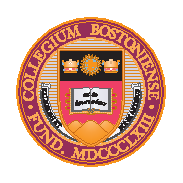
\includegraphics[width=0.5in]{BC-color.eps}}
%\end{minipage}
\titlegraphic{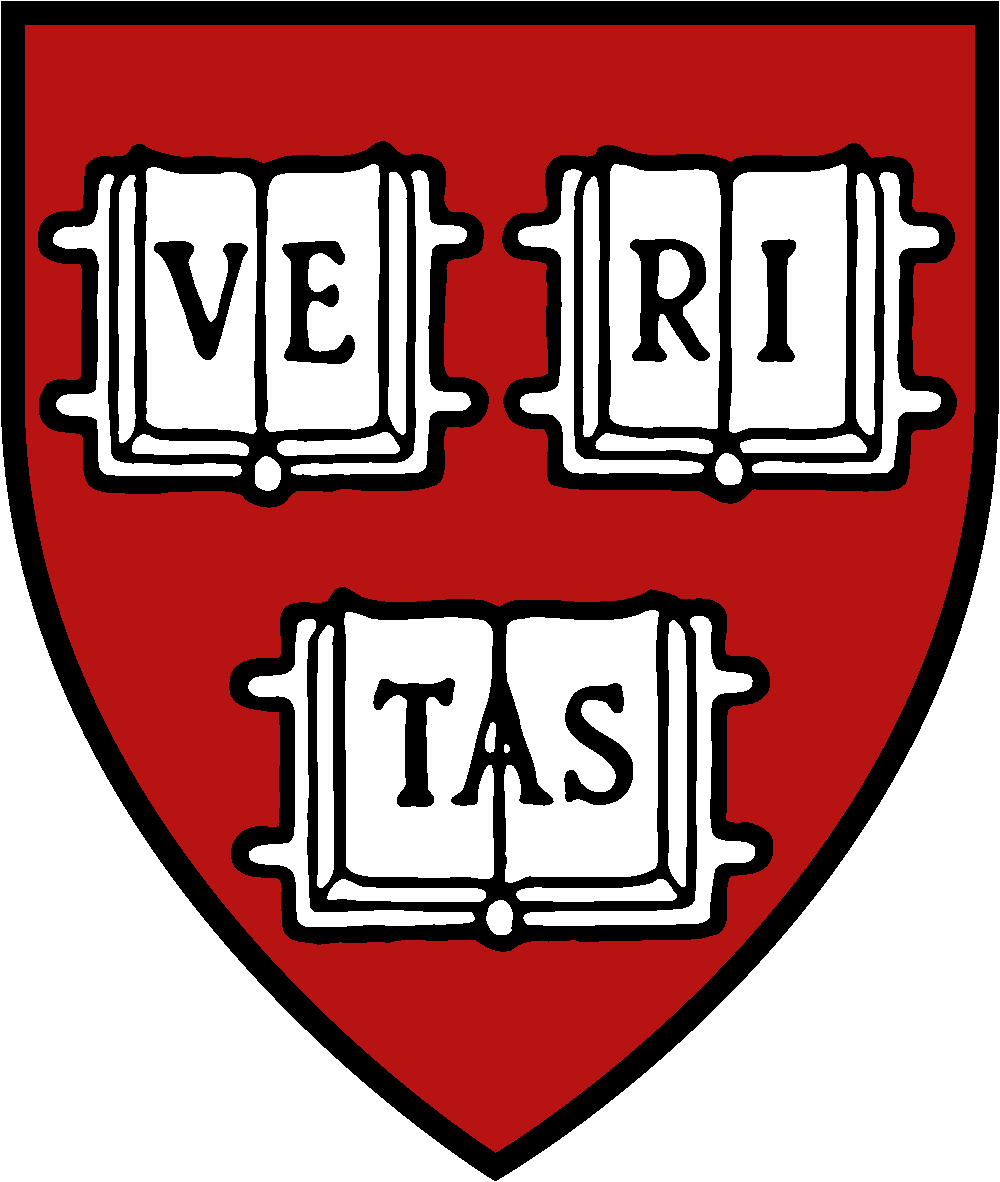
\includegraphics[height=0.5in]{Harvard.png}\hspace{0.3in}
\includegraphics[height=0.5in]{Stanford.png}\hspace{0.3in}
\includegraphics[height=0.5in]{UVIC.png}\hspace{0.3in}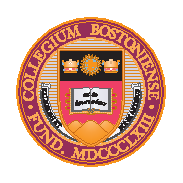
\includegraphics[height=0.5in]{BC-color.eps}}

\begin{frame}%[plain] % without section heads
	\titlepage
\end{frame}


\AtBeginSection[]{% add a frame of current position before every section
	\frame{
		\setcounter{tocdepth}{2}
		\frametitle{Contents}
		\tableofcontents[
			currentsection
		]
	}
}

\begin{frame}
	\frametitle{Outline}
	\tableofcontents
\end{frame}

%%%%%%%%%%%%%%%%%%%%%%%%%%%%%%%%%%%%%%%%%%%%%%%%%%%%%%%%%%%%%%%%%%%%%%%%%%%%%%%

\section{Nernst Experiments in Superconductors}
	\subsection{Nernst Effect}
		\begin{frame}\frametitle{Vortex Nernst Effect}
			\begin{columns}
				\begin{column}{0.5\textwidth}
					\begin{block}{Nernst Effect}
						Nernst signal $e_N$ is the detection of transverse electric field when a longitudinal thermal gradient $-\nabla T$ is applied
						\begin{equation*}
							e_N:=\dfrac{E_y}{-\partial_x T}.
						\end{equation*}
					\end{block}
					\only<2->{
					In a vortex-liquid state, longitudinal thermal gradient drives the motion of vortices. So Josphson equation
					\begin{equation*}
						2eV_J=\hbar \partial_t\varphi=2\pi\hbar \partial_t n_v
					\end{equation*}}
				\end{column}
				\begin{column}{0.4\textwidth}
					\begin{figure}[!htp]
						\centering
						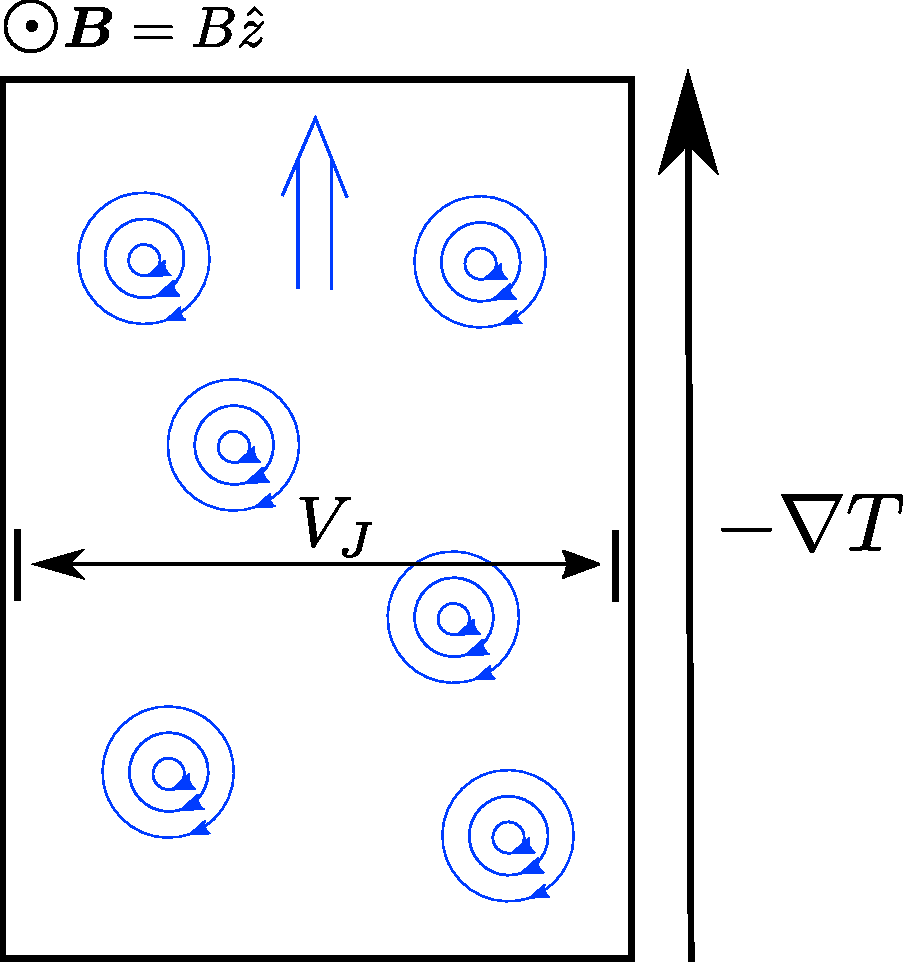
\includegraphics[scale=0.3]{vortex.pdf}
					\end{figure}
				\end{column}
			\end{columns}
			\only<2->{\hfill\par
			tells that \textbf{\color{red}the measured transverse voltage (or Nernst signal) is proportional to the density of vortices}.}
		\end{frame}

	\subsection{Experimental Results}
		\begin{frame}\frametitle{$\mathrm{La}_{2-x}\mathrm{Sr}_x\mathrm{CuO}_4$}
			\begin{columns}
				\begin{column}{0.45\textwidth}
					\begin{figure}[!htp]
						\centering
						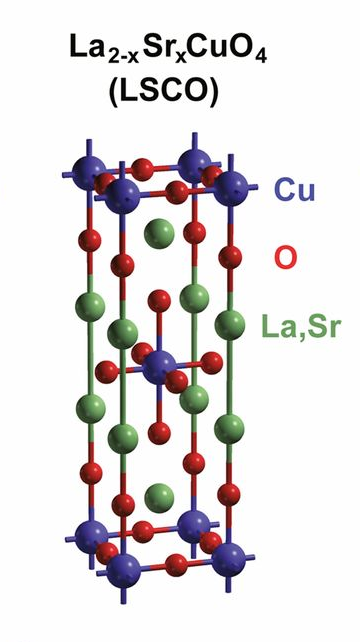
\includegraphics[scale=1]{SC.png}
						\caption{Extrated from {\scriptsize Barišić \textit{et al.} PNAS, \textbf{110}, 30 (2013)}.}
					\end{figure}
				\end{column}
				\begin{column}{0.45\textwidth}
					\begin{figure}[!htp]
						\centering
						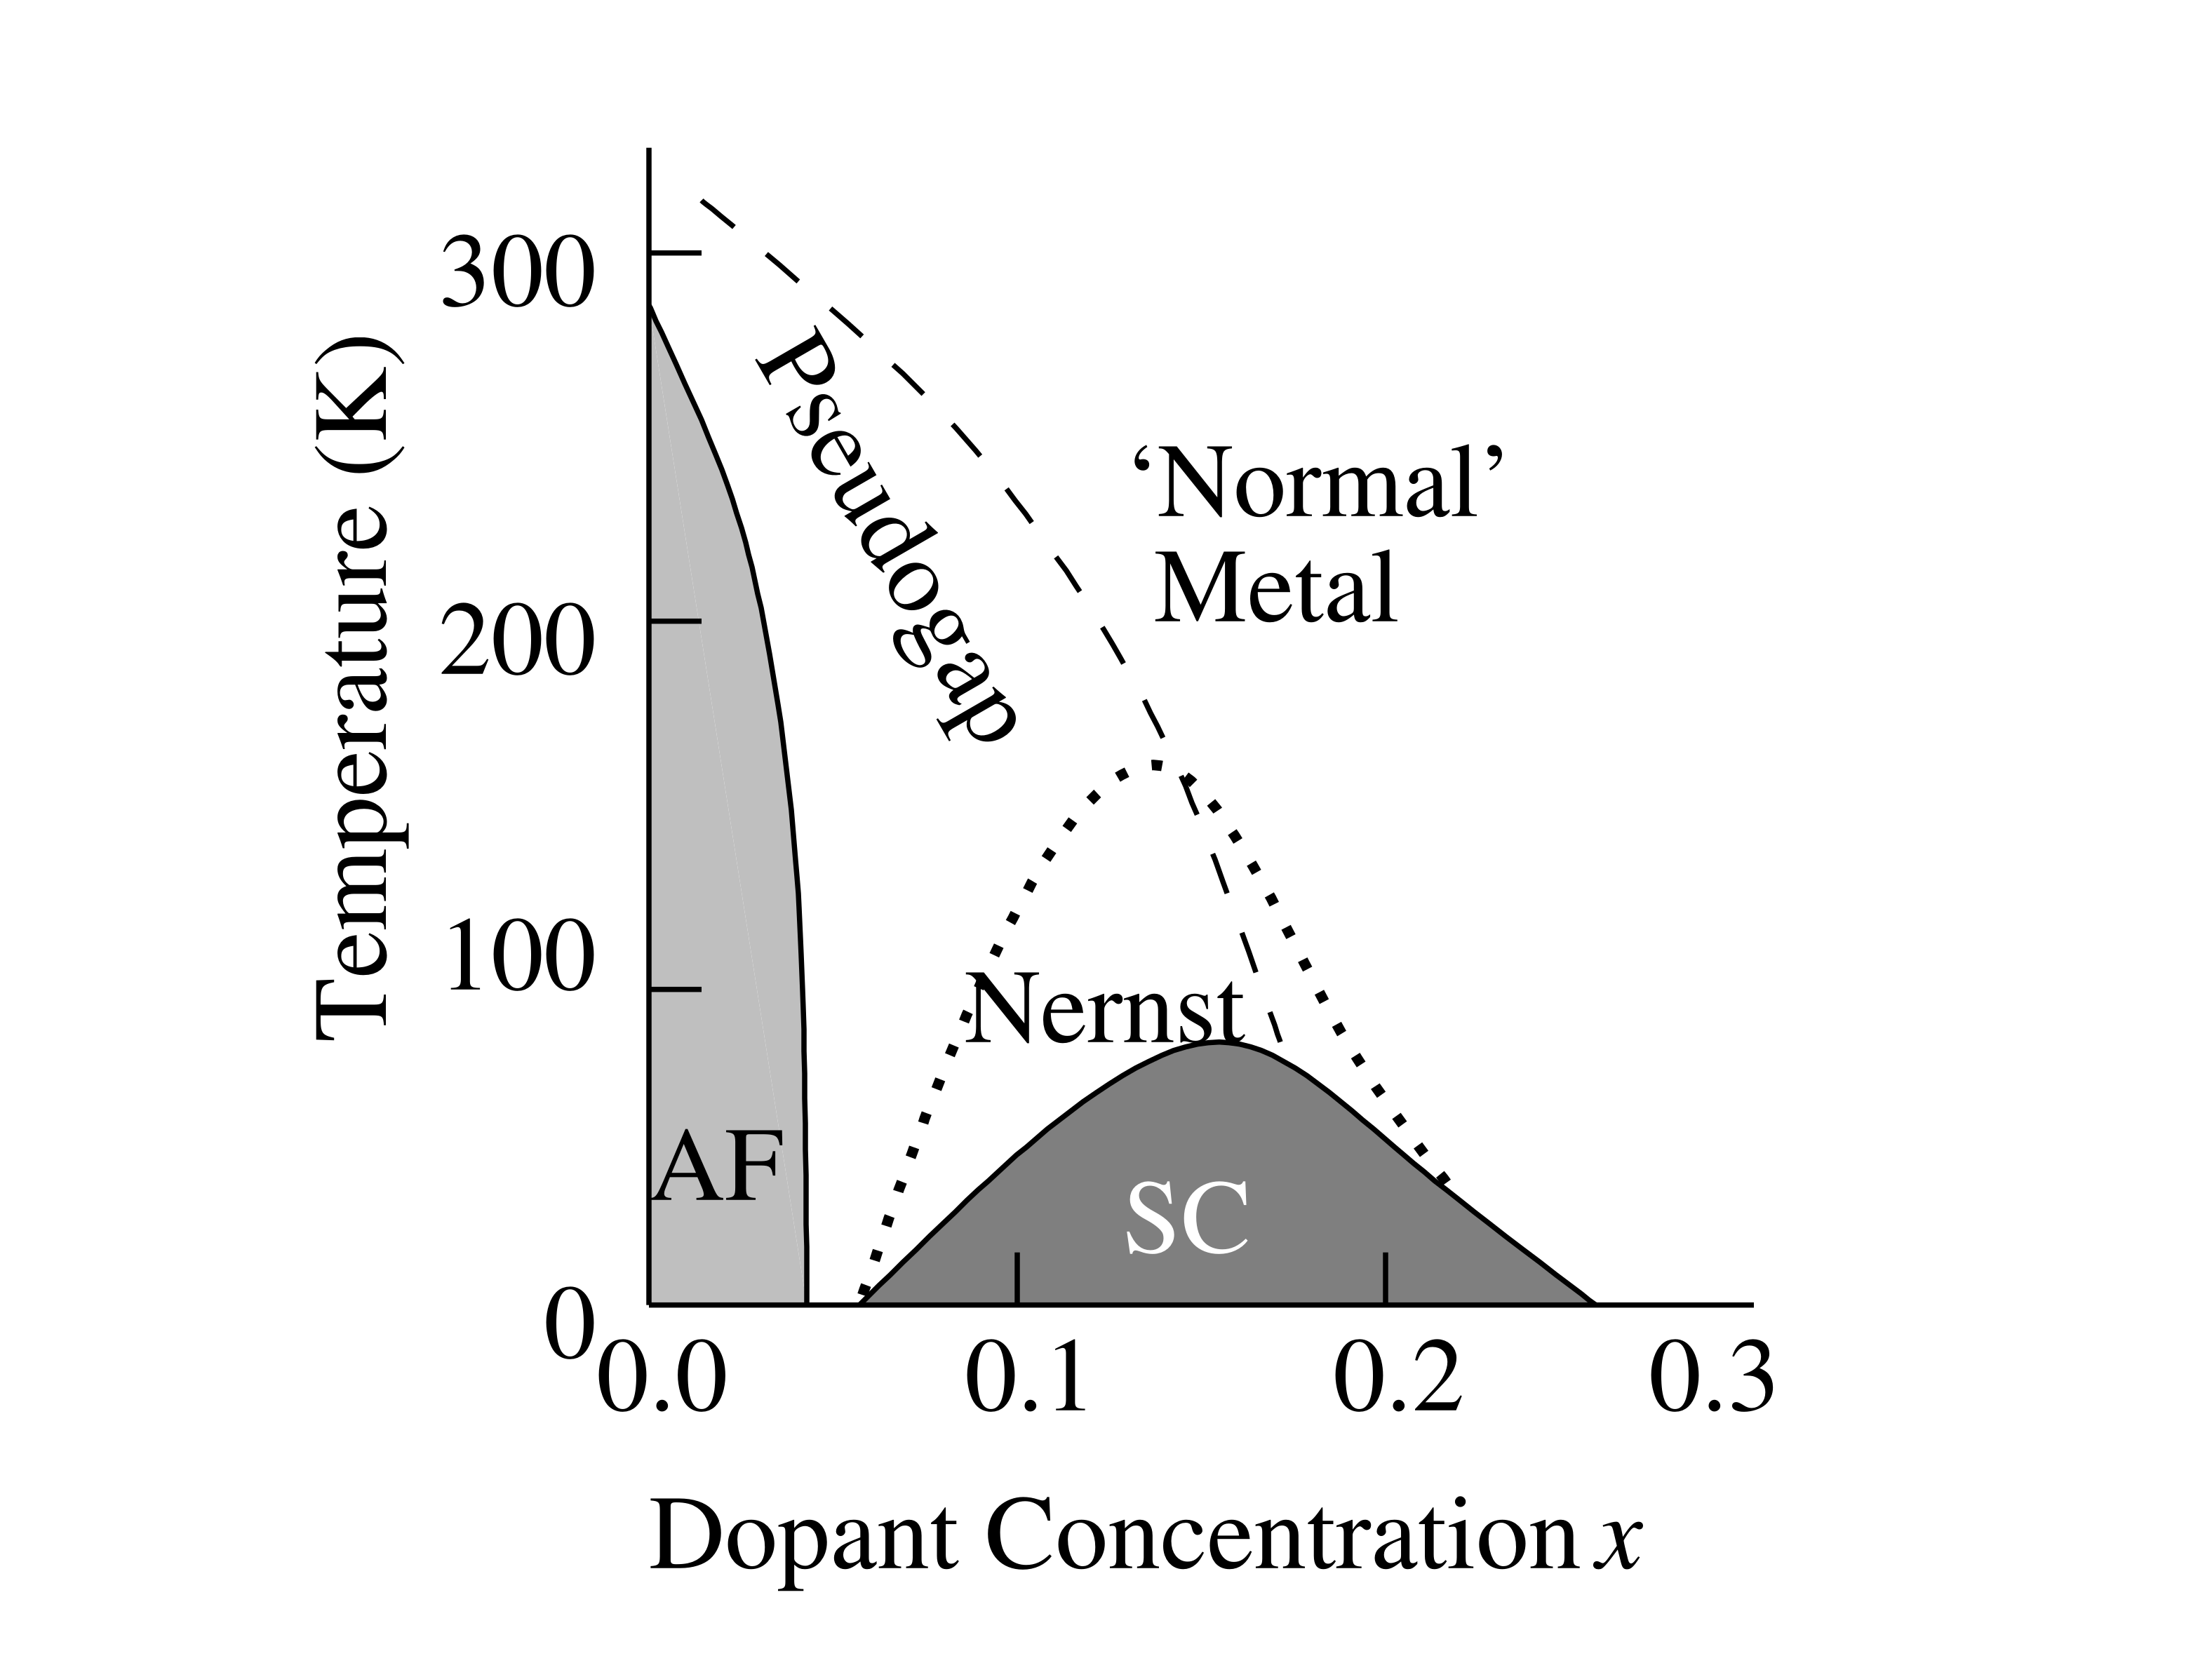
\includegraphics[scale=0.8]{Mott.png}
						\caption{\textbf{Phase Diagram of Dopped Mott Insulator}. Extrated from {\scriptsize Wen \textit{et al.} RMP, \textbf{28}, 1 (2006)}.}
					\end{figure}
				\end{column}
			\end{columns}
			
		\end{frame}
		
		\begin{frame}\frametitle{Nernst Region of LSCO}
			\begin{columns}
				\begin{column}{0.55\textwidth}
					\begin{figure}[!htp]
						\centering
						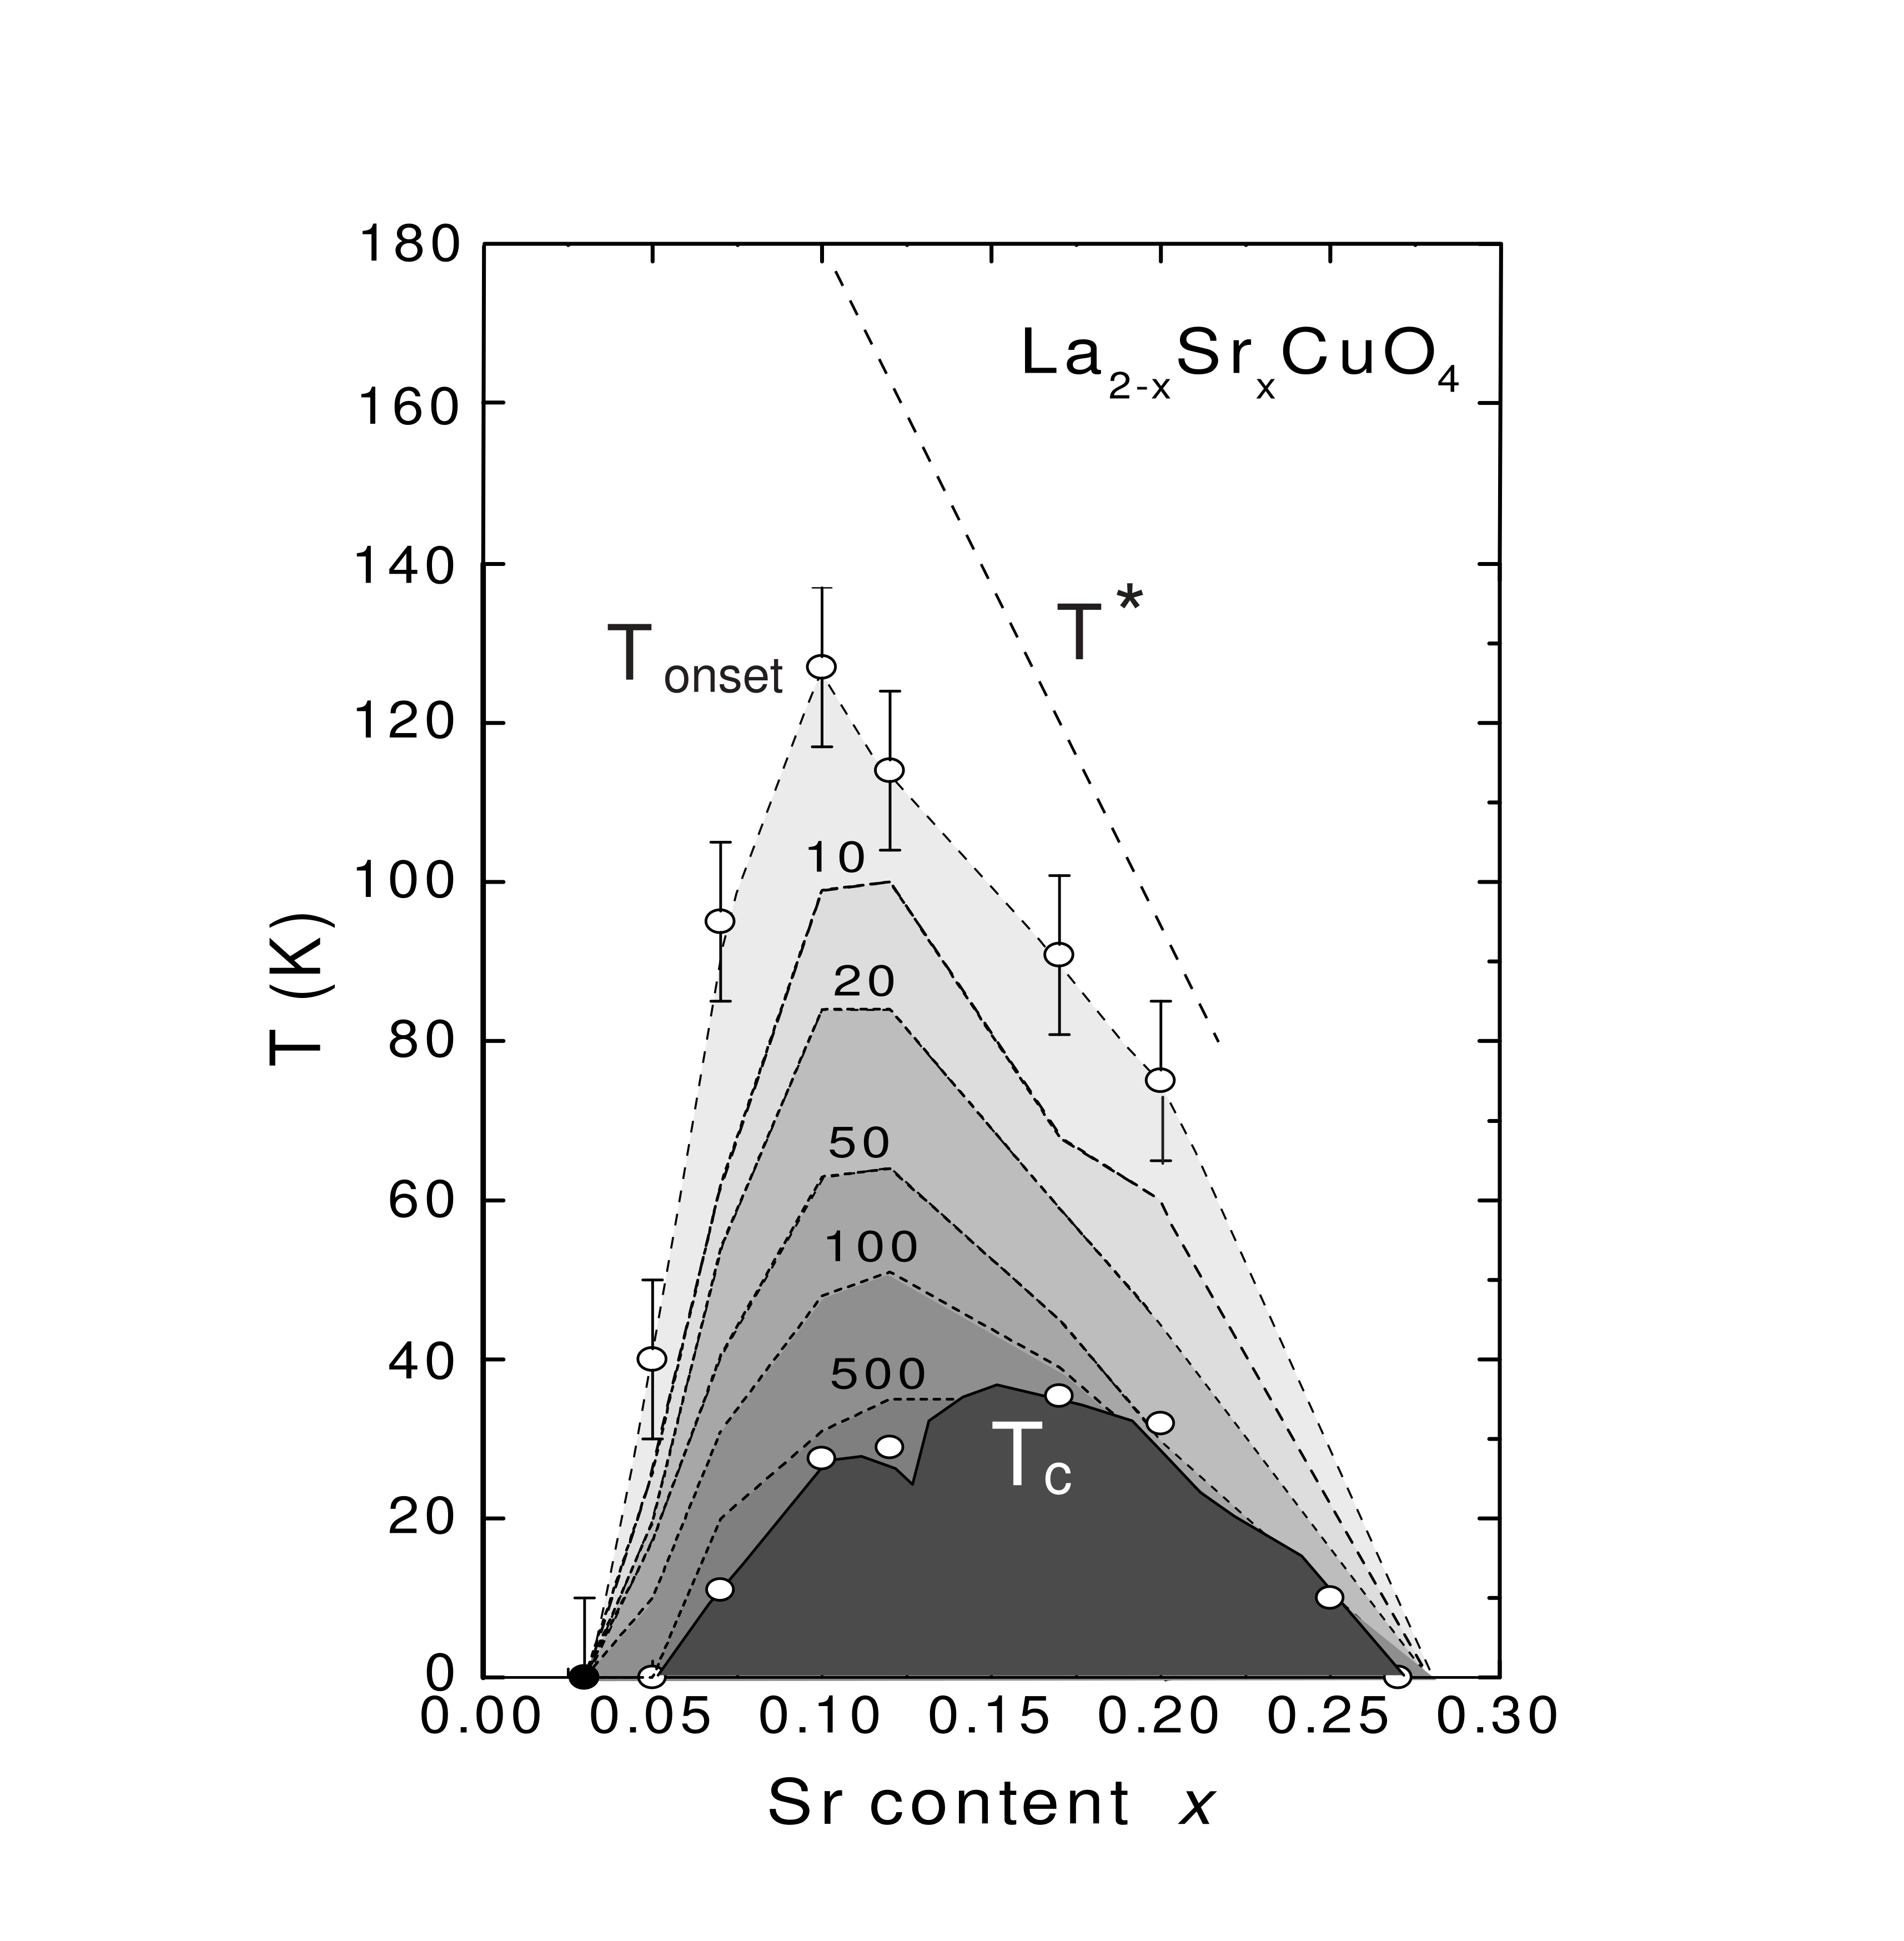
\includegraphics[scale=0.6]{LSCO.png}
						\caption{\textbf{Phase diagram of LSCO}. The Nernst coefficient on Contour $\nu\equiv e_N/B$. Extracted from {\scriptsize Wang \textit{et al.} PRB, \textbf{73}, 024510 (2006)}.}
					\end{figure}
				\end{column}
				\begin{column}{0.45\textwidth}
					\begin{figure}[!htp]
						\centering
						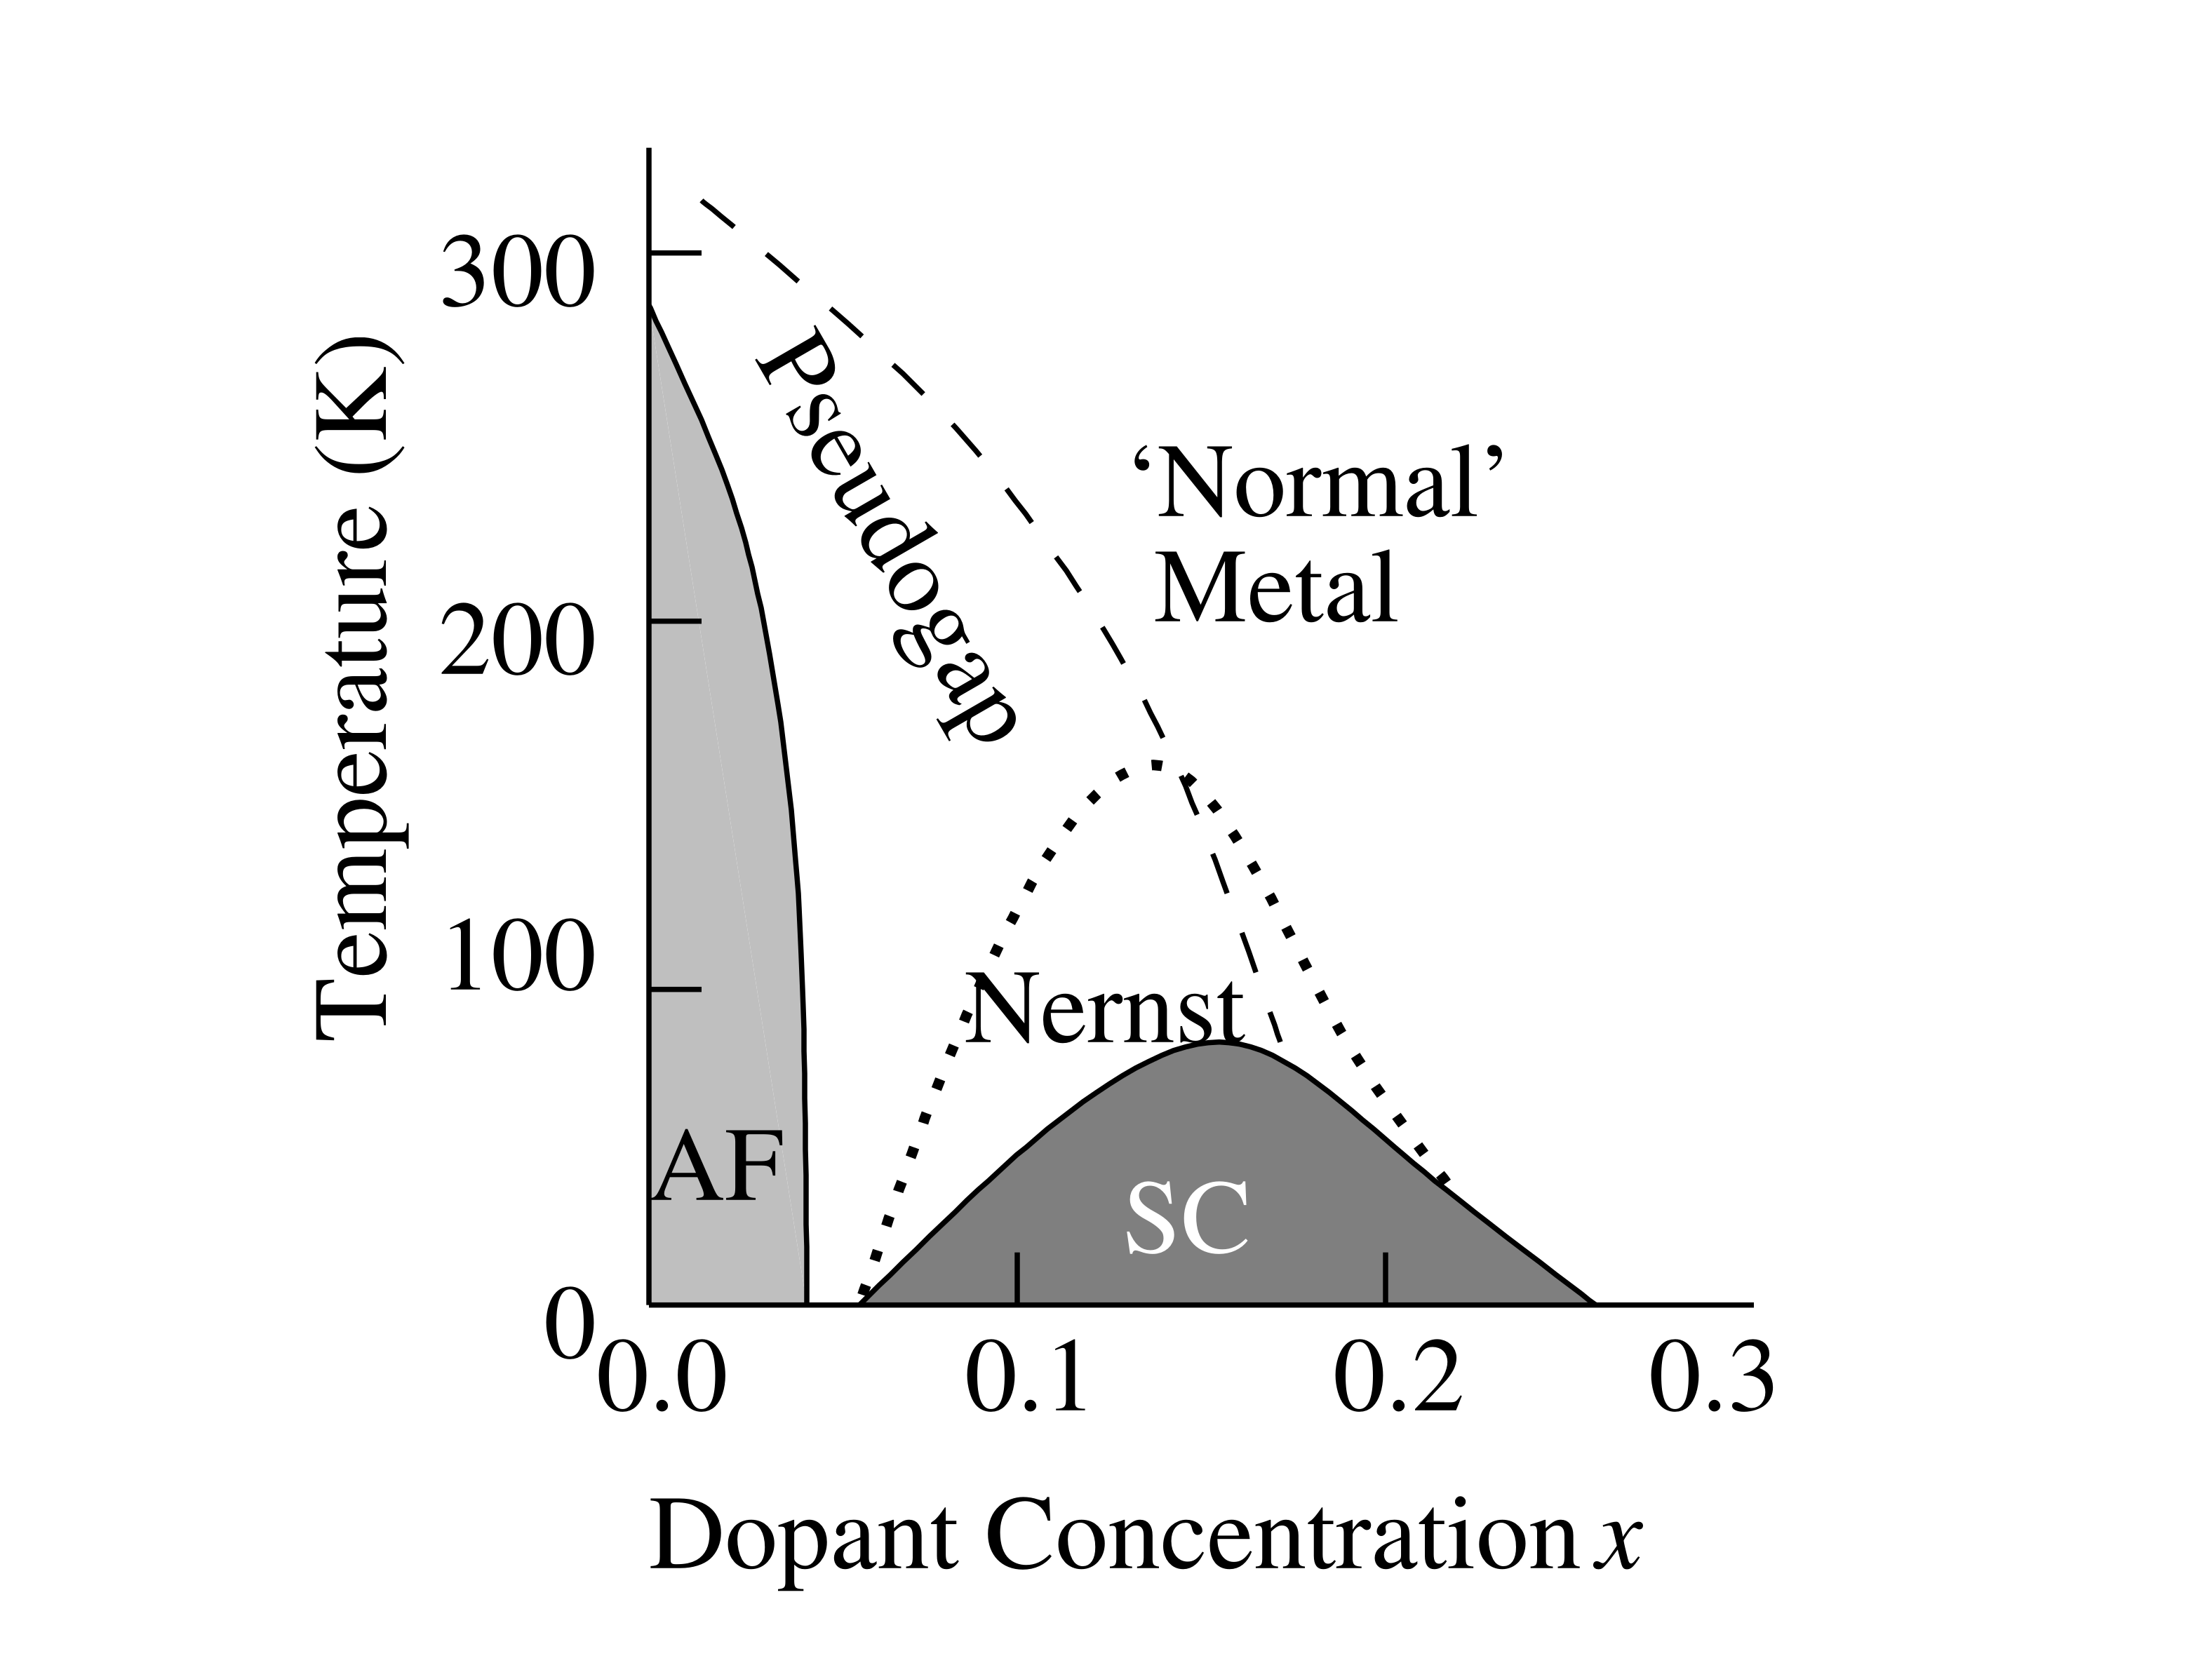
\includegraphics[scale=0.8]{Mott.png}
						\caption{\textbf{Phase Diagram of Dopped Mott Insulator}. Extrated from {\scriptsize Wen \textit{et al.} RMP, \textbf{28}, 1 (2006)}.}
					\end{figure}
				\end{column}
			\end{columns}			
		\end{frame}
		
		\begin{frame}\frametitle{Quantum Criticality}
			\begin{figure}[!htp]
				\centering
				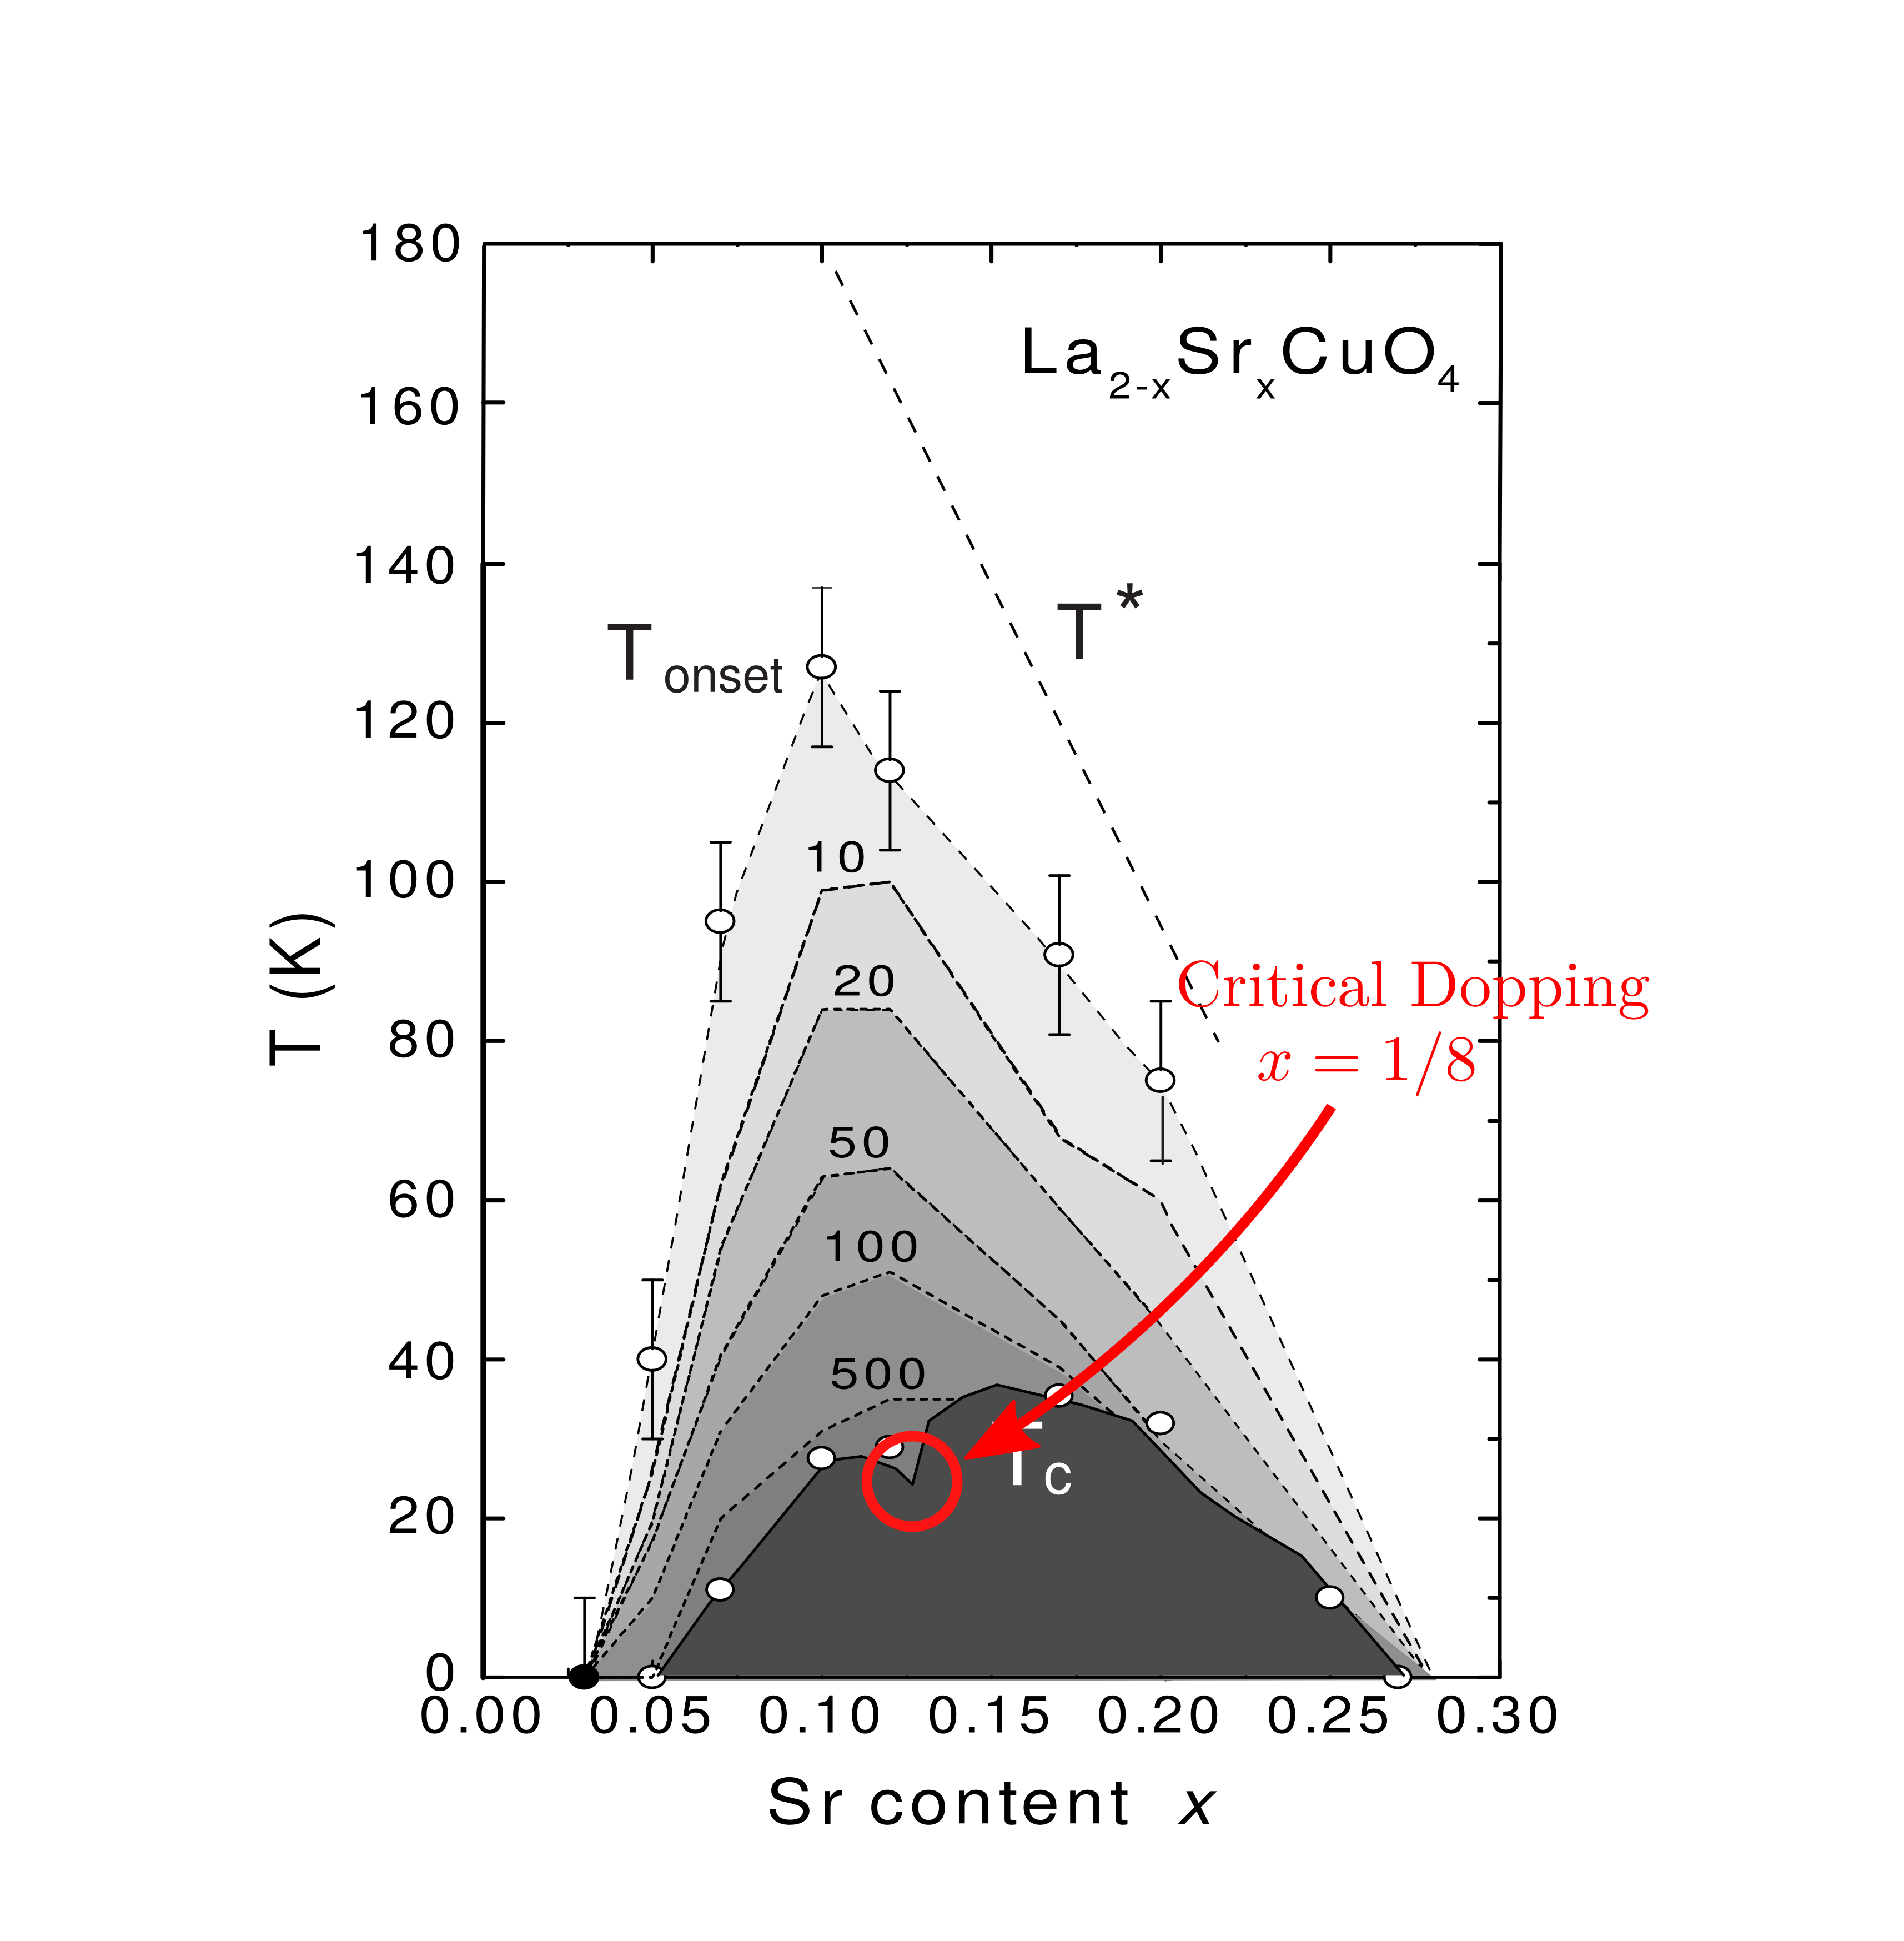
\includegraphics[scale=0.05]{LSCO-2.png}
				\caption{{\bf QCP}: The dip in $T_c$ near $x=1/8$ indicates proximity of Insulating Phase.}
			\end{figure}
		\end{frame}

\section{Relativistic Field Theory of Vortex Liquid}
	\subsection{Bose-Hubbard Model}
		\begin{frame}\frametitle{Bose-Hubbard Model}
			\begin{columns}
				\begin{column}{0.45\textwidth}
					The superconductor-insulator phase transition of vortices indicates
					\begin{block}{Bose-Hubbard Model}
						\begin{align*}
							H&=-t\sum_{\langle ij \rangle}b_i^\dagger b_j-\mu\sum_i n_i\\
							&\quad+\dfrac{U}{2}\sum_i n_i(n_i-1)
						\end{align*}
					\end{block}
				\end{column}
				\begin{column}{0.5\textwidth}
					\begin{figure}[!htp]
						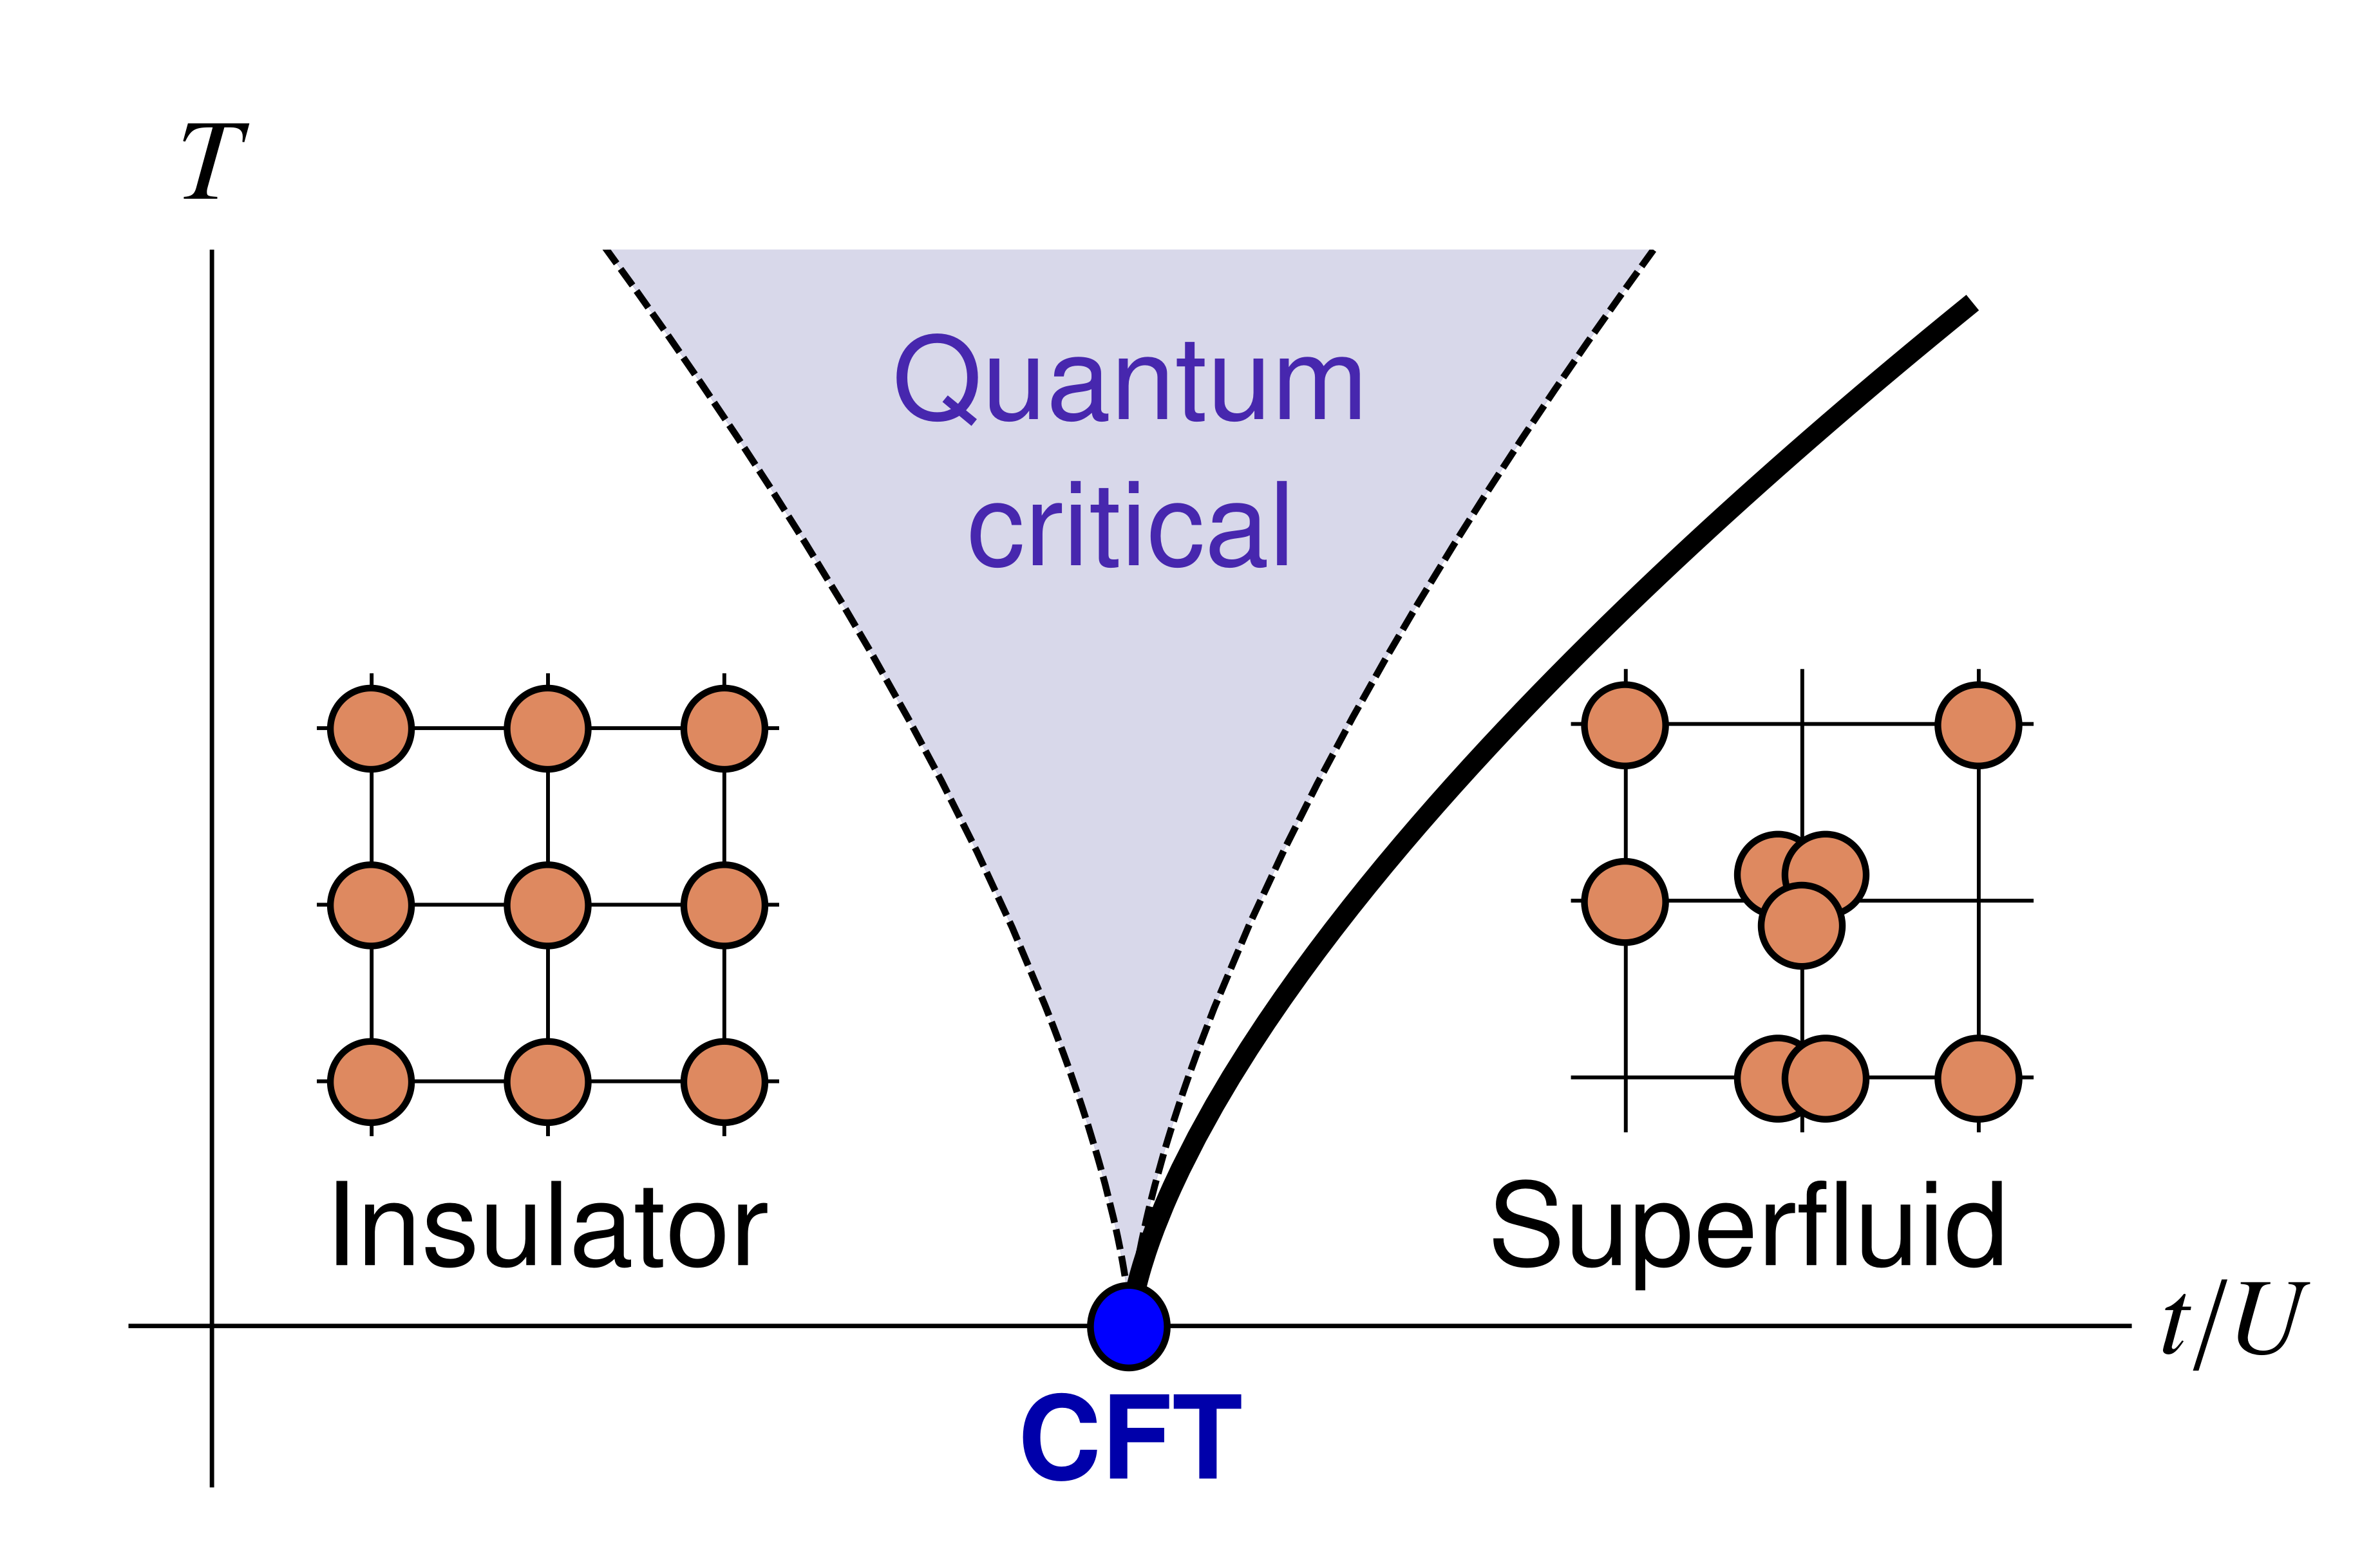
\includegraphics[scale=0.5]{Witczak.png}
						\caption{Extracted from {\scriptsize Witczak-Krempa \textit{et al.}, Nat. Phys., \textbf{10}, 5 (2014)}.}
					\end{figure}
				\end{column}
			\end{columns}
			\pause
			And the critical theory is given by ({\scriptsize Fisher \textit{et al.}, PRB, \textbf{40}, 1 (1989)})
			\begin{redblock}{(2+1)-D Conformal Field Theory}
				\begin{equation*}
					S=\int\dd^2r\dd\tau\bigg[|\partial_\tau\psi|^2+v^2|\nabla\psi|^2-g|\psi|^2+\dfrac{u}{2}|\psi|^4\bigg].
				\end{equation*}
			\end{redblock}
			%In the application of cuprates, the Mott insulator phase shrink to just one point of hole density $x=1/8$.
		\end{frame}

		\begin{frame}\frametitle{Linear Response Around Critical Point}
			\begin{columns}
				\begin{column}{0.45\textwidth}
					To study the Nernt effect of LSCO, we are going to perturb such CFT with 
					\begin{itemize}
						\item a (non-uniform) chemical potential $-\nabla\mu$
						\item a magnetic field $B$
						\item a (non-uniform) thermal fluctuation $-\nabla T$
					\end{itemize}
					and calculate the corresponding linear reponses.
				\end{column}
				\begin{column}{0.5\textwidth}
					\begin{figure}[!htp]
						\centering
						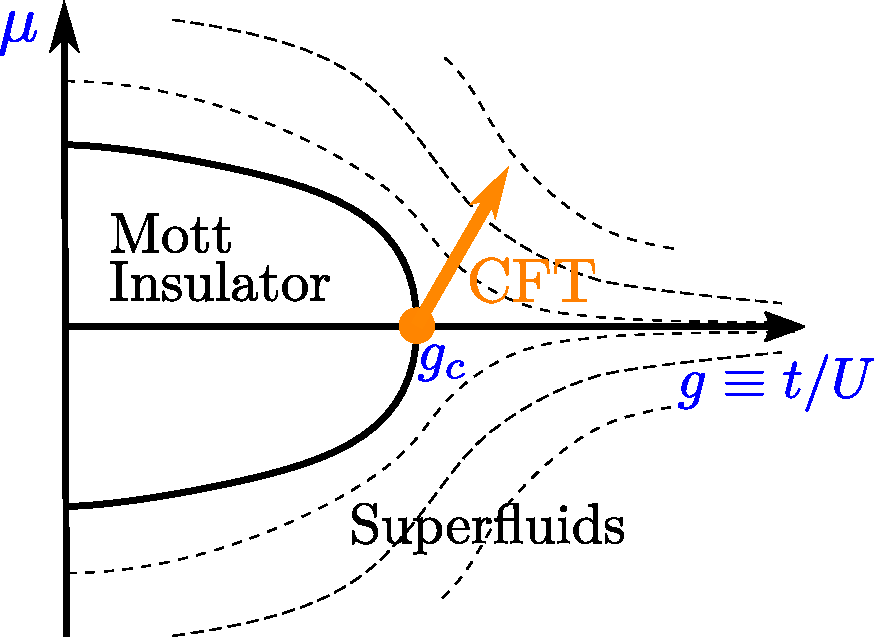
\includegraphics[scale=0.4]{CFT.pdf}
					\end{figure}
					
				\end{column}
			\end{columns}

			\begin{block}{Perturbative CFT}
				\begin{equation*}
					S=\int\dd^2r\dd\tau\bigg[|\partial_\tau-\mu\psi|^2+v^2|(\nabla-i\bm{A})\psi|^2-g|\psi|^2+\dfrac{u}{2}|\psi|^4\bigg].
				\end{equation*}
			\end{block}
		\end{frame}
		
\section{Relativistic Hydrodynamics}
	\subsection{Constitutive Relation}		
		\begin{frame}\frametitle{Conservation Law}
			The Lorentz-invariant microscopic action gives two macroscopic \textbf{Ward identities} ({\scriptsize Herzog, J. Phys. A, \textbf{42}, 34 (2009)}) (as \textbf{\color{red}conservation laws})
			\begin{redblock}{Conservation Laws}
				\begin{equation*}
					\nabla_\mu\langle T^{\mu\nu}\rangle=F^{\nu\lambda}\langle J_\lambda\rangle,\quad \partial_\mu\langle J^\mu\rangle=0,
				\end{equation*}
			\end{redblock}
			where
			\begin{itemize}
				\item (macroscopic) current operator $\langle J^\mu\rangle\equiv-\dfrac{\delta}{\delta A_\mu}W[g,A]$,
				\item (macroscopic) stress-energy tensor $T^{\mu\nu}\equiv=\dfrac{-2}{\sqrt{-g}}\dfrac{\delta}{\delta g_{\mu\nu}}W[g,A]$,
				\item $W[g,A]$ is the generating functional (with explicit dependence on metric tensor and vector potential).
			\end{itemize}
		\end{frame}
		
		\begin{frame}\frametitle{What is Hydrodynamics in Condensed Matter Physics?}
			Landau and Lifshitz (1959) first proposed the modern version of hydrodynanics. The basic assumptions of hydrodynamics are
			\begin{greenblock}{Assumption}
				\begin{itemize}
					\item The long-wave length physics is dominated by very limited number of variables (called hydro-variables), which are nothing but the \textbf{conserved ones}.\\
					$\implies$ Up to the physical length scale, \textbf{\color{red}all physical observables are determined by those hydro-variables}.
					\item The concrete from of those functionals are contrained merely by the \textbf{local version} of the second law of thermodynamics---non-negativity of entropy production.
				\end{itemize}
			\end{greenblock}
			\pause
			In our theory, the set of hydro-variables are $\{u^\mu, T, \mu\}$, where velocity vector $u^\mu$ is normalized up to the speed of light $u_\mu u^\mu\equiv-1$.
		\end{frame}
		

		\begin{frame}\frametitle{Constitutive Relation --- Zeroth Order}
			By {\scriptsize Eckart, Phys. Rev., \textbf{58}, 10 (1940)}, given a vector $u^\mu$, one can always decompose the two tensors with the projection operator $\mathcal{P}^{\mu\nu}=g^{\mu\nu}+u^\mu u^\nu$ that
			\begin{align*}
				J^\mu&=\mathcal{N}u^\mu+j^\mu,\\
				T^{\mu\nu}&=\mathcal{E}u^\mu u^\nu+\mathcal{P}P^{\mu\nu}+(q^\mu u^\nu+q^\nu u^\mu)+t^{\mu\nu},
			\end{align*}
			where scalar $\mathcal{N}$, $\mathcal{E}$, and $\mathcal{P}$, vector $j^\mu$ and $q^\nu$, and tensor $t^{\mu\nu}$ are formally contractions with whether velocity vector or projection operator.
			\pause
			Choosing the proper frame of reference, one has
			\begin{block}{Zeroth Order}
				\begin{equation*}
					\mathcal{N}=n(T,\mu),\quad \mathcal{E}=\varepsilon(T,\mu)+P(T,\mu),\quad\mathcal{N}=P(T,\mu).
				\end{equation*}
			\end{block}
			so that \textbf{\color{red}the entropy current is conserved $\partial_\mu s^\mu\equiv \partial_\mu (su^\mu)=0$}, or \textbf{in equilibrium}.
		\end{frame}
		

		\begin{frame}\frametitle{Constitutive Relation --- First Order}
			Choosing the \textbf{Landau frame} (1959) for the proper definition of \textbf{\color{red}out-of-equilibrium} thermodynamic variables, and using the property of \textbf{time-reversal symmetry} and \textbf{parity-inversion symmetry}, we can write down the most general combinations of those functionals
			\begin{block}{First Order}
				\begin{align*}
					j^\mu&=-\sigma_Q TP^{\mu\nu}\partial_\nu\left(\dfrac{\mu}{T}\right)-\chi_T P^{\mu\nu}\partial_\nu T,\\
					\mathcal{P}&=P-\zeta \partial_\lambda u^\lambda,\\
					q^\mu&=0,\\
					t^{\mu\nu}&=-\eta P^{\mu\alpha}P^{\nu\beta}\bigg(\partial_\alpha u_\beta+\partial_\beta u_\alpha-\dfrac{2}{2}g_{\alpha\beta}\partial_\lambda u^\lambda\bigg).
				\end{align*}
			\end{block}
			\pause
			The non-trivial constraint of entropy production requires
			\begin{equation*}
				\chi_T\equiv0,\quad \zeta>0,\quad \sigma_Q>0,\quad\eta>0. 
			\end{equation*}
		\end{frame}

	\subsection{Linear Response}
		\begin{frame}\frametitle{Hydrodynamic EOM}
			Following {\scriptsize Kandanoff\&Martin, Ann. Phys., \textbf{24}, 419 (1969)}, the linear response over equilibrium state can be obtained by introducing a purtabative Hamiltonian
			\begin{equation*}
				\mathcal{H}\rightarrow\mathcal{H}-\int\dd^{2}x\,\left(\dfrac{\delta T}{T}(\varepsilon-\mu\rho)+\delta \mu\rho+\delta u^\mu T_{\mu0}\right),
			\end{equation*}
			where we explicitly split out the perturbative source of energy density, charge density, and momentum densities.\\
			\pause
			Linearized Hydrodynamic equations of motion are read out from conservation laws
			\begin{block}{Conservation Laws}
				\begin{align*}
					\partial_t\rho+\nabla\cdot\bigg\{\rho\bm{v}+\sigma_Q\left[-\nabla\mu+\dfrac{\mu}{T}\nabla T+\bm{v}\times\bm{B}\right]\bigg\}&=0\\
					\partial_t\varepsilon+\nabla\cdot\bigg((\varepsilon+P)\bm{v}\bigg)&=0\\
					\partial_t\bigg((\varepsilon+P)\bm{v}\bigg)+\nabla p-\zeta\nabla(\nabla\cdot\bm{v})-\eta\nabla^2\bm{v}-\delta\bm{J}\times B&=0.
				\end{align*}
			\end{block}
		\end{frame}

		\begin{frame}\frametitle{Thermoelectric Response}
			The full thermoelectric response			
			\begin{equation*}
				\left(\begin{array}{c}
					\bm{J}\\\bm{Q}
				\end{array}\right)=\left(\begin{array}{cc}
					\bm{\sigma}&\bm{\alpha}\\T\bm{\alpha}&\bm{\bar{\kappa}}
				\end{array}\right) \left(\begin{array}{c}
					-\nabla\mu\\-\nabla T
				\end{array}\right) 
			\end{equation*}
			can be obtained after a lengthy calculation, with the poles
			\begin{block}{\textbf{Cyclotron Resonance}}
				\begin{equation*}
					\omega=\pm\omega_c+i\gamma,\quad \omega_c\equiv\dfrac{v^2}{c^2}\dfrac{2B}{(\varepsilon+P)/\rho c},\quad \gamma\equiv\sigma_Q\dfrac{v^2}{c^2}\dfrac{B^2}{\varepsilon+P}.
				\end{equation*}
			\end{block}
			\pause
			We are also interested in 
			\begin{itemize}
				\item heat current induced by thermal gradient but in the absence of charge current $\bm{Q}=-\bm{\kappa}\nabla T$. So $\bm{\kappa}\equiv\bm{\bar{\kappa}}-T\bm{\alpha}\bm{\sigma}^{-1}\bm{\alpha}$,
				\item electric field induced by thermal gradient but in the absense of charge current $\bm{E}=-\bm{\theta}\nabla T$. So $\bm{\theta}\equiv-\bm{\sigma}^{-1}\bm{\alpha}$.
			\end{itemize}
		\end{frame}

		\begin{frame}\frametitle{Thermoelectric Response}
			On the aspect of ``particle'',
				\begin{align*}
					\sigma_{xx}&=\sigma_Q\dfrac{\omega+i\gamma+i\omega_c^2/\gamma}{(\omega+i\gamma)^2-\omega_c^2},&\sigma_{xy}&=-\dfrac{\rho}{B}\dfrac{\gamma^2+\omega_c^2-2i\gamma\omega}{(\omega+i\gamma)^2-\omega_c^2},\\
					\alpha_{xx}&=\dfrac{\rho}{T}\dfrac{i\omega}{(\omega+i\gamma)^2-\omega_c^2},&\alpha_{xy}&=-\dfrac{\gamma}{B}\dfrac{\gamma^2+\omega_c^2-i\gamma\omega}{(\omega+i\gamma)^2-\omega_c},\\
					\bar{\kappa}_{xx}&=s\dfrac{i\omega-\gamma}{(\omega+i\gamma)^2-\omega_c^2},&\bar{\kappa}_{xy}&=-s\dfrac{\omega_c}{(\omega+i\gamma)-\omega_c^2},
				\end{align*}
			while on the aspect of ``vortex'',
			\begin{align*}
				\rho_{xx}&=\dfrac{1}{\sigma_Q}\dfrac{\omega(\omega+i\omega_c^2/\gamma+i\gamma)}{(\omega+i\omega_c^2/\gamma)-\omega_c^2},&\rho_{xy}&=\dfrac{B}{\rho}\dfrac{(\omega_c^2/\gamma)^2+\omega_c^2-2i(\omega_c^2/\gamma)\gamma\omega}{(\omega+i\omega_c^2/\gamma)^2-\omega_c^2},\\
				\theta_{xx}&=\dfrac{s}{\rho}\dfrac{(\omega_c^2/\gamma)^2+\omega_c^2-i(\omega_c^2/\gamma)\omega}{(\omega+i\omega_c^2/\gamma)^2-\omega_c^2},&\theta_{xy}&=-\dfrac{B}{T}\dfrac{i\omega}{(\omega+i\omega_c^2/\gamma)-\omega_c^2},\\
				\kappa_{xx}&=s\dfrac{i\omega-\omega_c^2/\gamma}{(\omega+i\omega_c^2/\gamma)-\omega_c^2},&\kappa_{xy}&=s\dfrac{\omega_c}{(\omega+i\omega_c^2/\gamma)-\omega_c^2}.
			\end{align*}
		\end{frame}


\section{Results}
	\subsection{Self Duality}
		\begin{frame}\frametitle{Byproduct: Nontrivial Self Duality}
			Under the interchange of $\rho\leftrightarrow B$ and $\sigma_Q\leftrightarrow 1/\sigma_Q$, the cyclotron resonance remain unchanged and $\gamma\leftrightarrow\gamma_v\equiv\omega_c^2/\gamma$. And we observe an amazing self duality that
			\begin{redblock}{Particle-Vortex Duality}
				\begin{equation*}
					\xymatrix{\sigma_{xx}, \sigma_{xy}, \alpha_{xx}, \alpha_{xy}, \bar{\kappa}_{xx}, \bar{\kappa}_{xy} \ar@2{<->}[d] \\ \rho_{xx},-\rho_{xy},-\theta_{xy},-\theta_{xx},\kappa_{xx},-\kappa_{xy},}
				\end{equation*}
			\end{redblock}
			which is believed to have a close relation with M-theory, see {\scriptsize Herzog \textit{et al.}, PRD, \textbf{75}, 8 (2009)}.
		\end{frame}

	\subsection{Comparison with Experiments}
		\begin{frame}\frametitle{Nernst Signal} 
			In the presence of momentum relaxation (characterized by $\tau$), the measured Nernst signal corresponds to the transverse component
			\begin{equation*}
				e_N\equiv\theta_{yx}=\dfrac{k_B}{2e}\dfrac{\varepsilon+P}{k_B T\rho}\left[\dfrac{\omega_c/\tau}{(\omega_c^2/\gamma+1/\tau)+\omega_c^2}\right].
			\end{equation*}
			Using the previous study of temperature dependence of thermodynamics quantities near the critical point ({\scriptsize Chubukov \textit{et al.}, PRB, \textbf{49}, 17 (1994)} and {\scriptsize Sachdev (1994)}) that
			\begin{equation*}
				\varepsilon=k_BT\left(\dfrac{k_BT}{\hbar v}\right)^2\Phi_\varepsilon,\quad P=k_BT \left(\dfrac{k_B T}{\hbar v}\right)^2\Phi_P, 
			\end{equation*}
			where $\Phi_\varepsilon$ and $\Phi_P$ are dimensionless numbers, we can plot $e_N$ as a function of temperature $T$ and magnetic field $B$ and compare that with experiments.
		\end{frame}
		
		\begin{frame}\frametitle{Comparison}
			\only<1>{
			\begin{itemize}
				\item Taking a typical scatter time $\tau\sim 10^{-12} \mathrm{s}$, we can estimate the velocity using simply Drude formula such that $\hbar v=47 \mathrm{meV\cdot\AA}$. This value is in accordance with experimental ranges (see {\scriptsize Balasky \textit{et al.}, Science, \textbf{284}, 5417 (1999)}). 
				\item We can also calculate $\Phi_\varepsilon$ and $\Phi_P$ with $\varepsilon$-expansion ({\scriptsize Damle \textit{et al.}, PRB, \textbf{56}, 8714 (1997)}). Up to single-loop level $\Phi_s+\Phi_P=4\pi^2/45$. 
			\end{itemize}}
			\only<2->{\begin{columns}
				\begin{column}{0.45\textwidth}
					\begin{figure}[!htp]
						\centering
						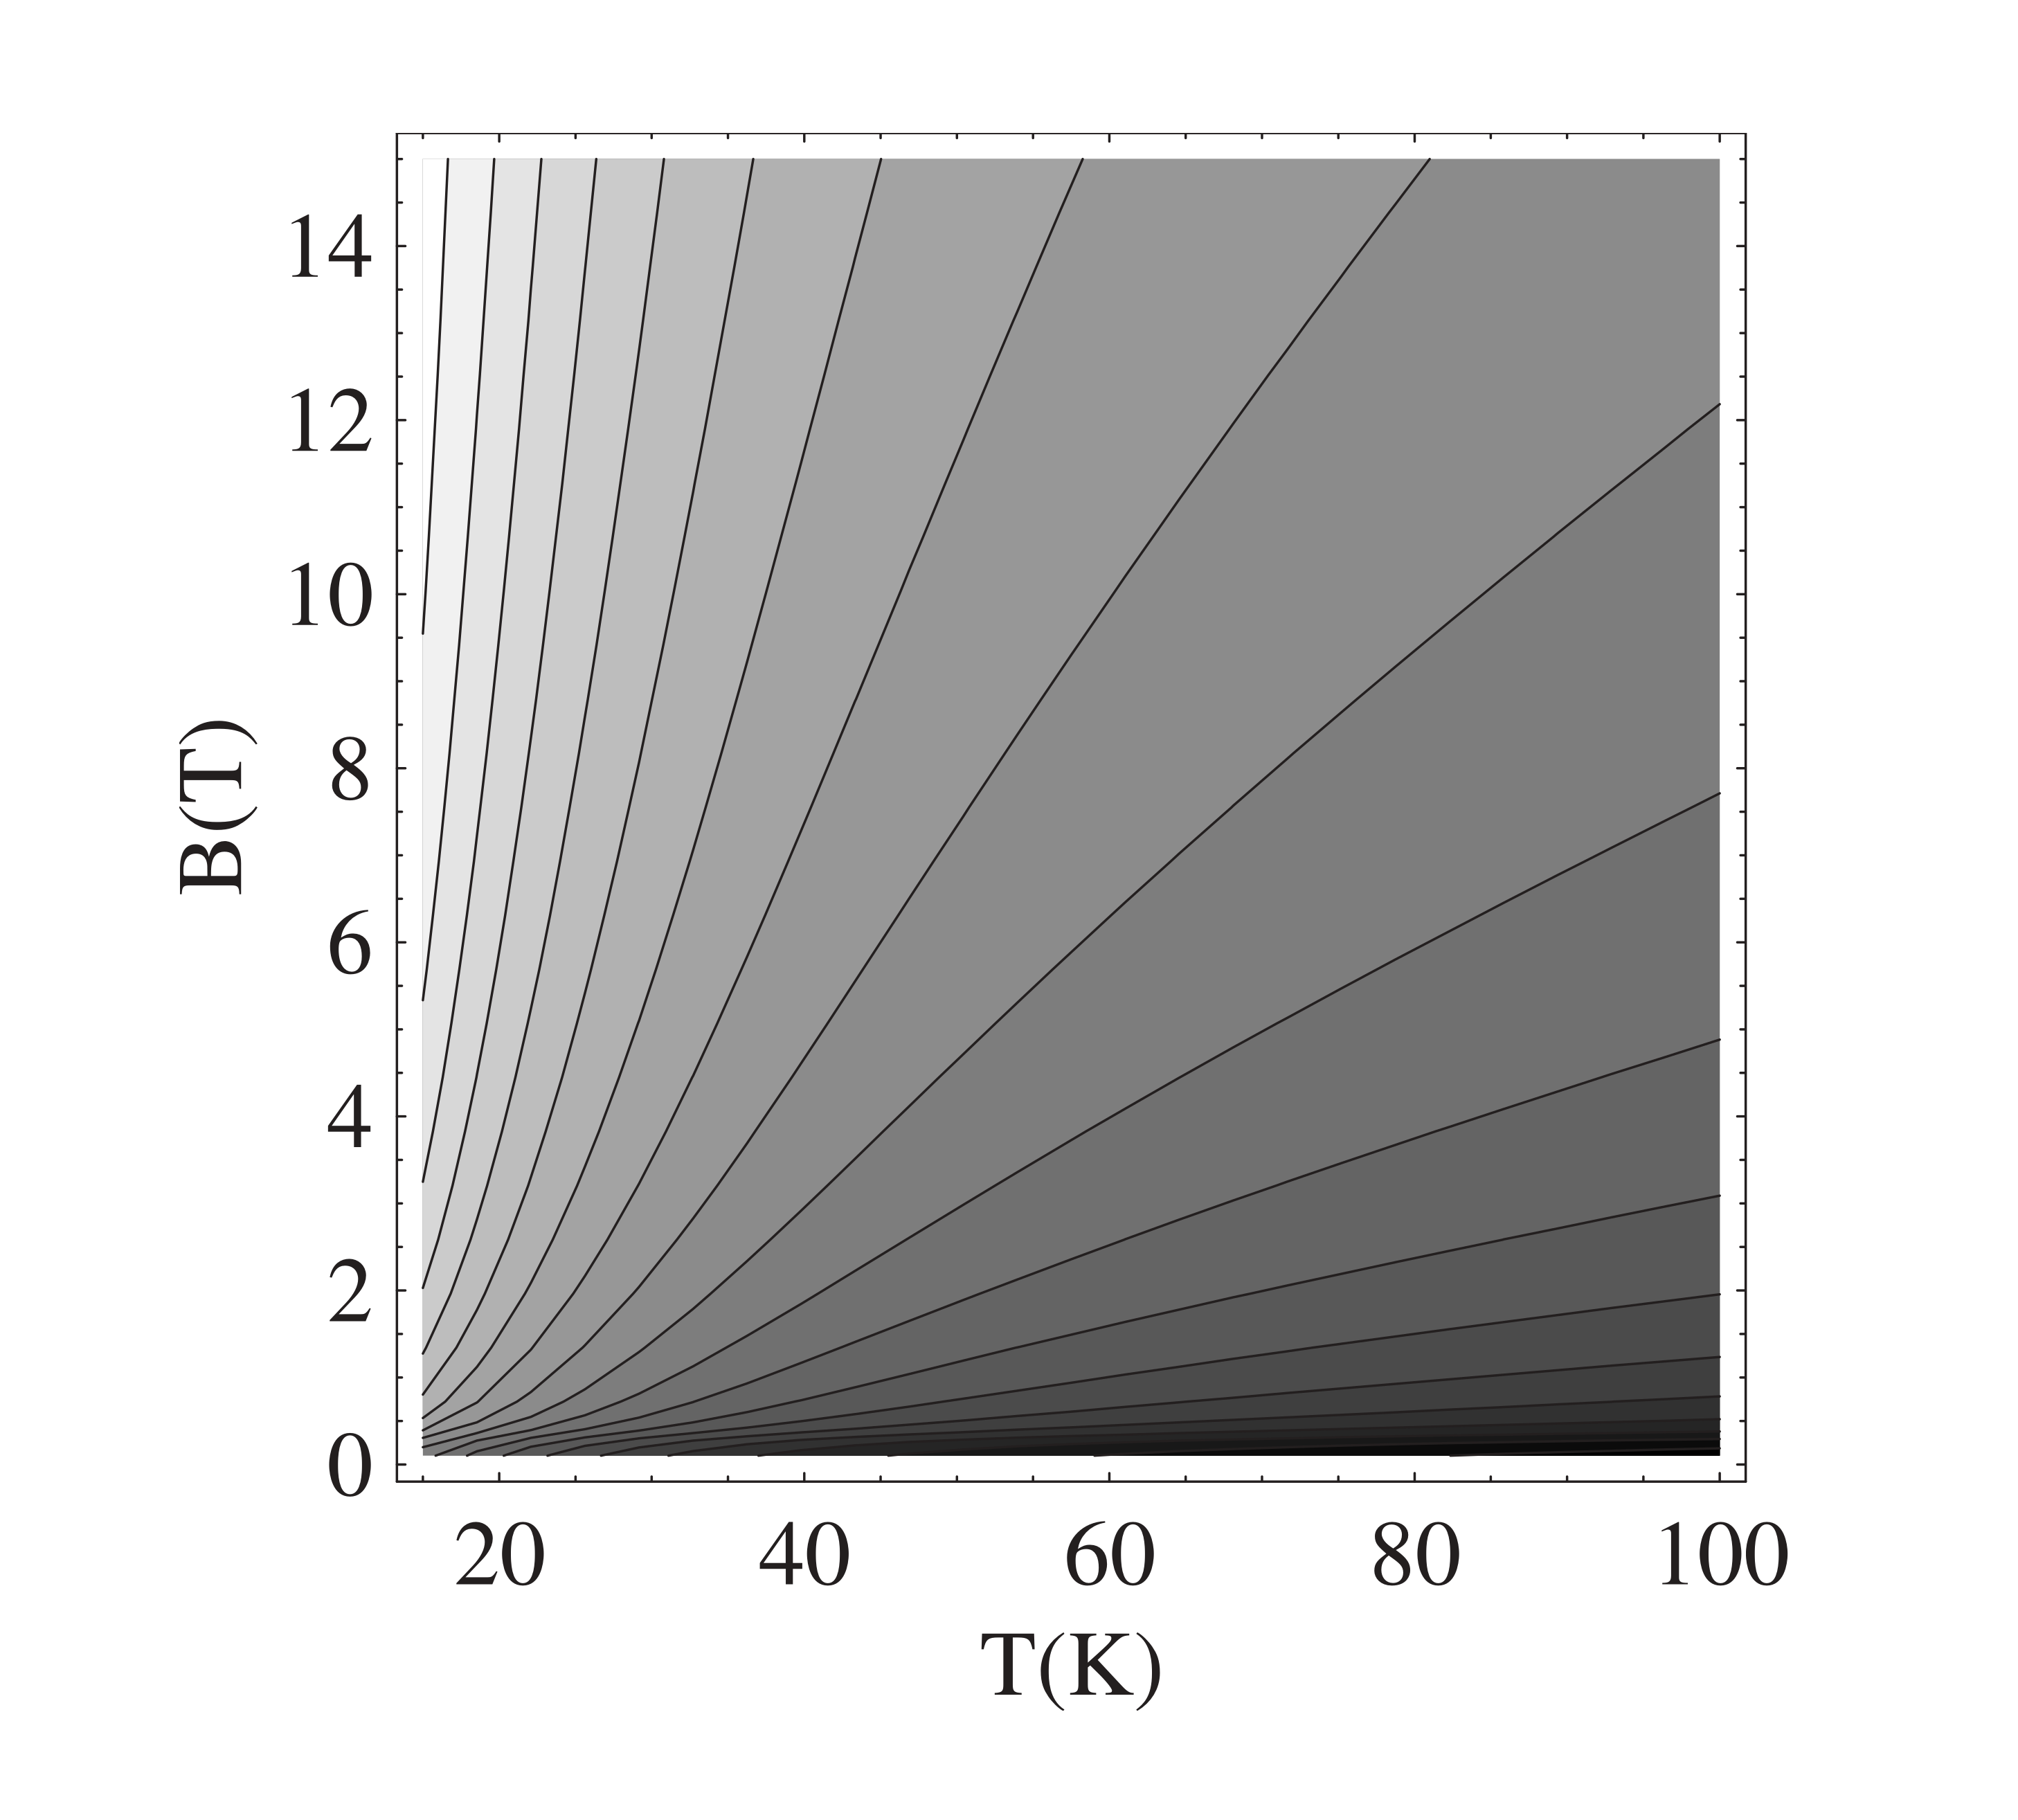
\includegraphics[scale=0.6]{eN.png}
						\caption{Calcualted $e_N(B,T)$. Extracted from {\scriptsize Hartnoll \textit{et al.}, PRB, \textbf{76}, 144502 (2007)}.}
					\end{figure}
				\end{column}
				\begin{column}{0.45\textwidth}
					\begin{figure}[!htp]
						\centering
						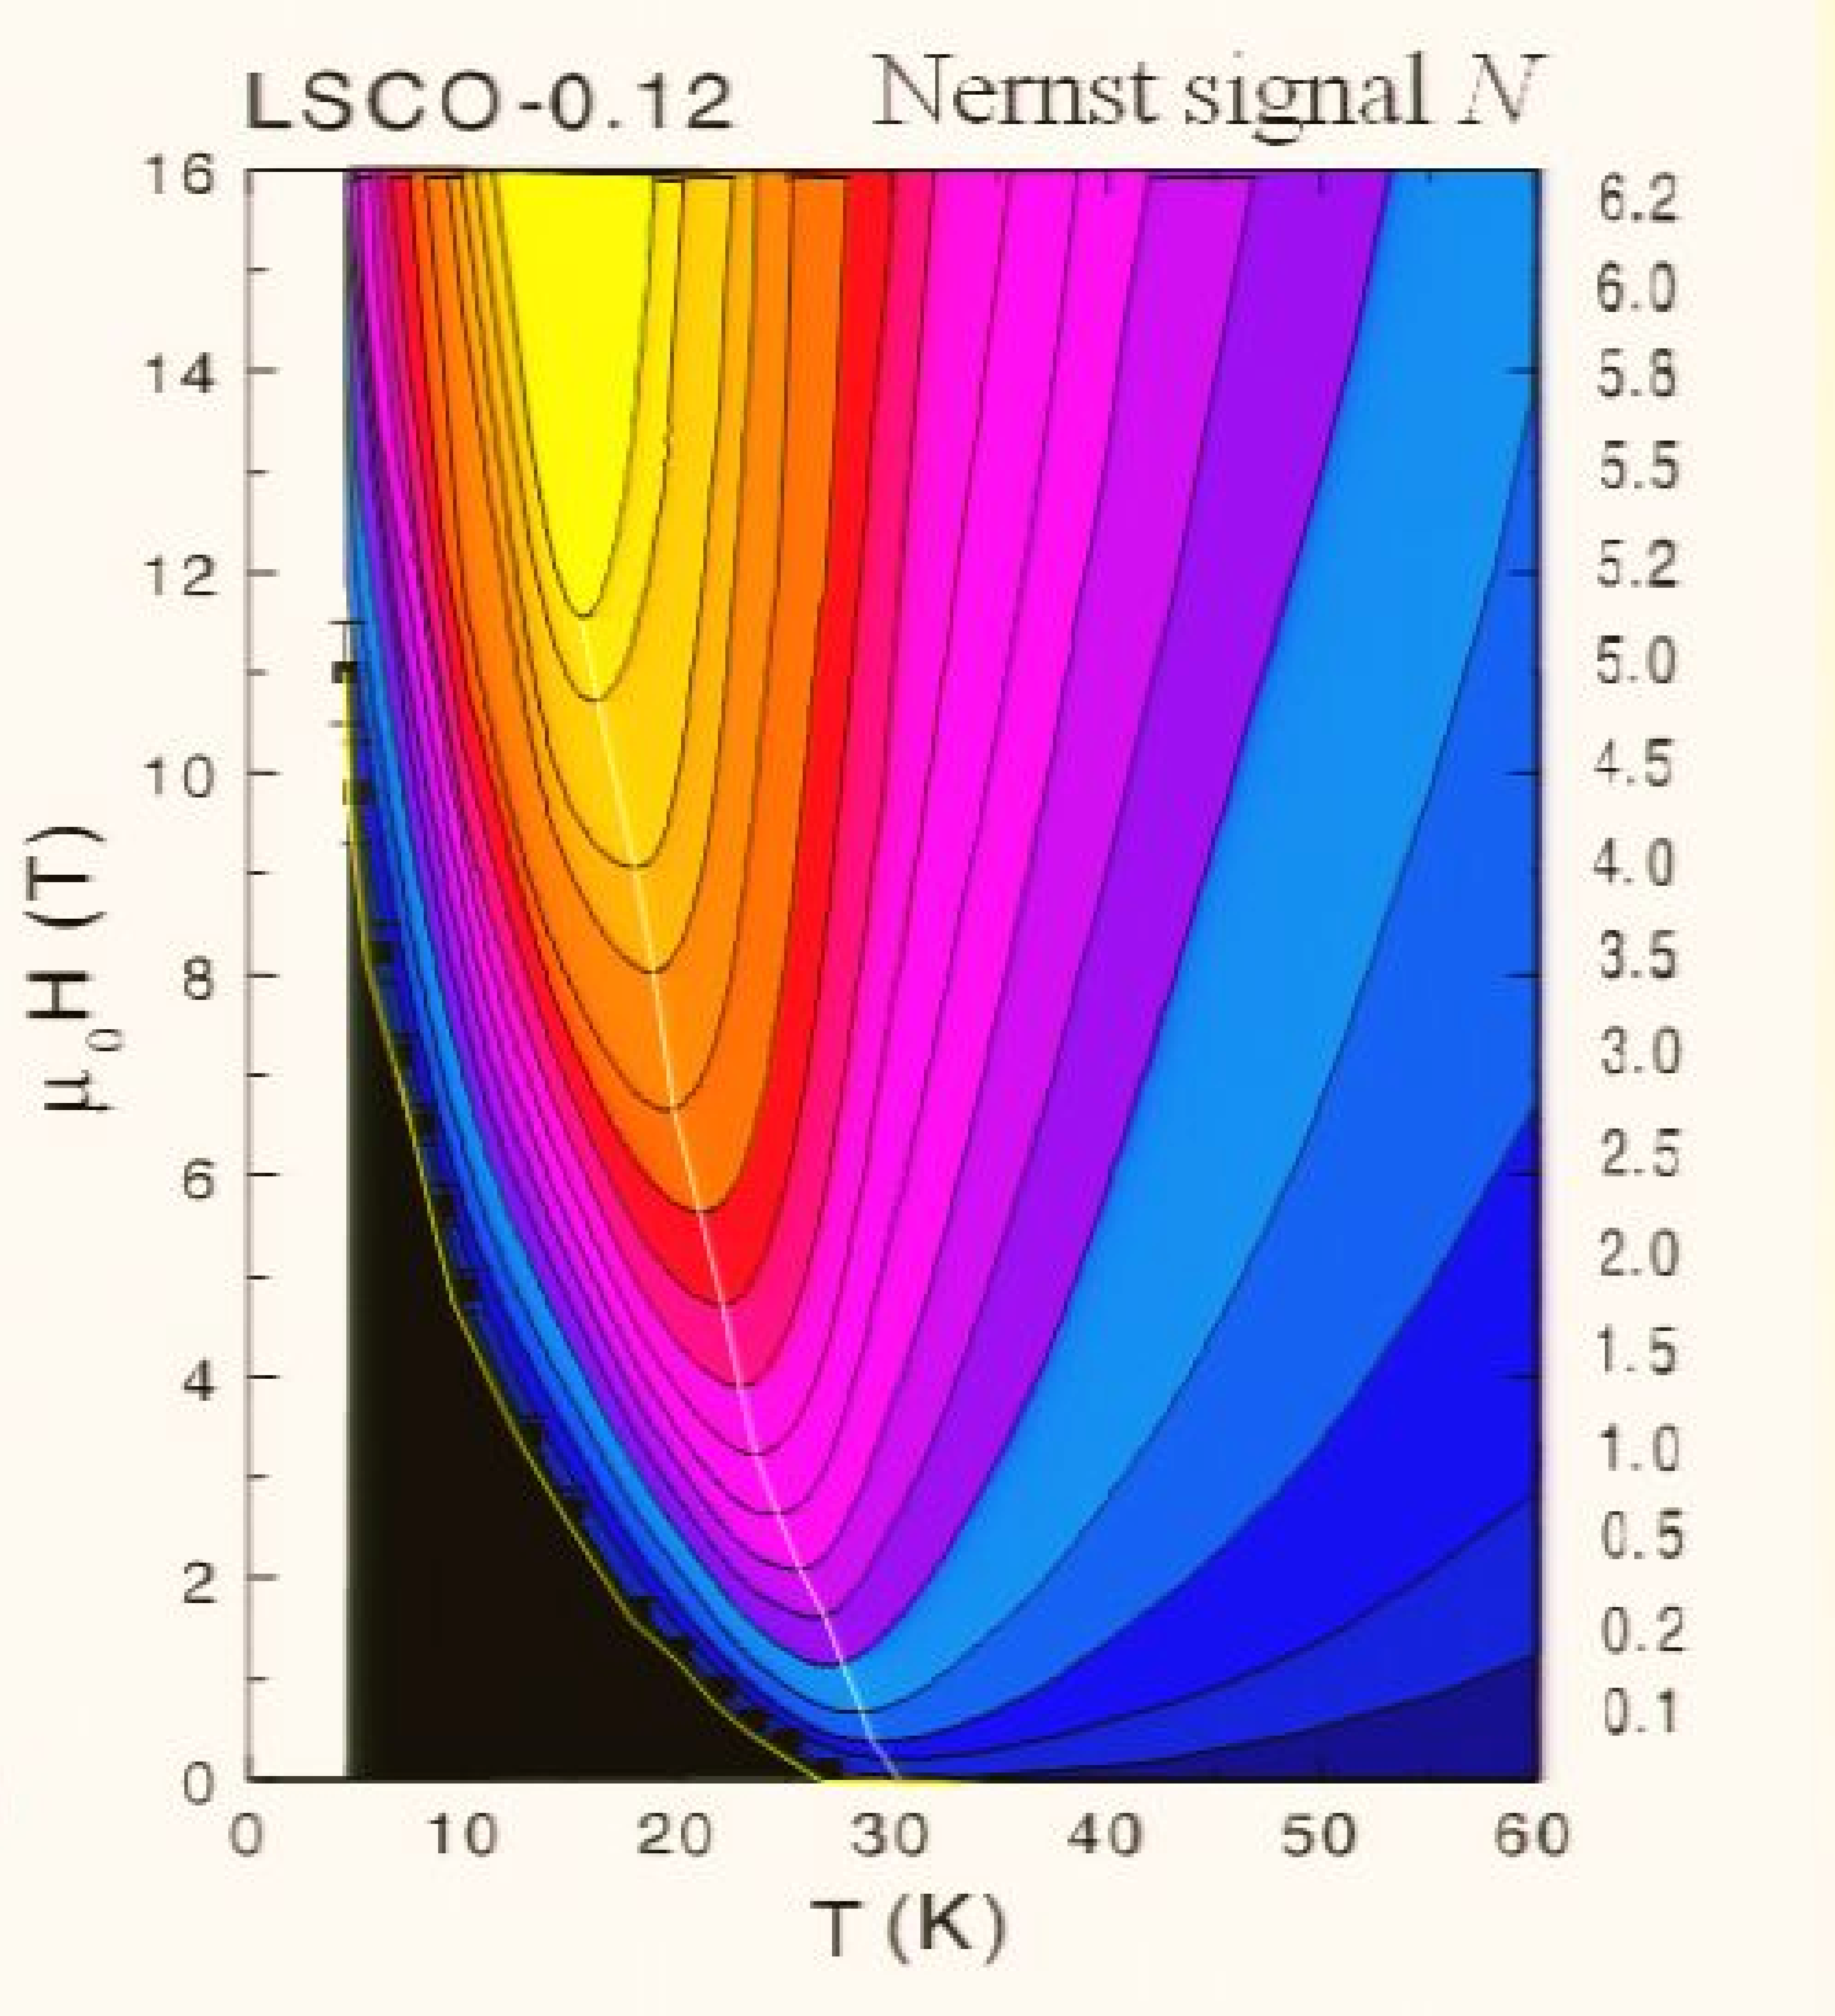
\includegraphics[scale=0.3]{Wang.png}
						\caption{Measured $e_N(B,T)$. Extracted from {\scriptsize Wang \textit{et al.}, PRL, \textbf{88}, 25 (2002)}.}
					\end{figure}
					
				\end{column}
			\end{columns}}
		\end{frame}
		
		
\section{Summary}
	\begin{frame}\frametitle{Summary}
		\begin{itemize}
			\item We propose a relativistic low-energy effecive field theory around the critical region of LSCO.
			\item We use hydrodynamic theory to obtain all thermoelectric coefficients.
			\item We find a realizaion of particle-vortex duality on transport coefficients.
			\item We estimate the phase diagram of Nernst signal and find it matches with the experimental data. 
		\end{itemize}
		\only<2>{
			\begin{center}
				\Huge Thanks!
			\end{center}
		}
	\end{frame}



\end{document}
